\documentclass[3p]{elsarticle}
%\documentclass[preprint]{revtex4-1}
\usepackage{amsmath, amsfonts, amssymb, bm, graphicx}
\usepackage{algorithm2e, nicefrac}

\title{Fluid plasma simulations with cut-cell adaptive mesh refinement}

%For els
%\author[sintef]{Robert Marskar}
%\ead{robert.marskar@sintef.no}
%\address[sintef]{SINTEF Energy Research}

\def\diff{\ensuremath{\text{d}}}
\def\bmx{\ensuremath{\bm{x}}}
\def\bmu{\ensuremath{\bm{u}}}
\def\bmi{\ensuremath{\bm{i}}}

\begin{document}
\begin{abstract}
A parallelized computational framework for planar two- and fully three-dimensional plasma fluid simulations of gaseous electrical discharges is investigated. Our approach uses cut-cell, multilevel grids with embedded boundaries for accurately describing electrode and dielectric surfaces. The plasma equation are then solved in space by using finite volume methods over this discretization, and are then evolved transiently using linear multistep methods. Numerical examples of two- and three-dimensional propagation in centimeter-sized gaps are then provided, with an emphasis on the formalism used. 
\end{abstract}
\maketitle

\section{Introduction}
Streamers are non-thermal, self-propagating weakly ionized plasma filaments with bright (i.e. radiating) heads and are precursors to electrical sparks, sprites, and lightning. A streamer moves as an ionization wave due to space-charge screening of the plasma filament and electron impact ionization in the streamer head that leads to self-enhancement of the electric field at the tip fo the filament.

Computational modelling of propagating weakly ionized plasmas is inherently difficult due to length scales that differ by several orders of magnitude. For example, in air at atmospheric pressure the plasma filament is surrounded by a space-charge layer with a thickness of tens to hundreds of micrometers, while the streamer itself can propagate tens of centimeters. Such large aspect ratios set particularly stringent requirements on the spatial grid. The presence of numerical stiffness in the equations of motion further complicates numerical modeling. In the plasma modeling community, it is commonly accepted that adaptive mesh refinement (AMR) is required for numerically resolving such phenomena, especially in three dimensions. The inclusion of internal boundary conditions, such as electrodes and dielectric materials inside the computational domain leads to additional numerical complexities, and it essential that these are resolved in a way that remain compatible with AMR. 

%%, and may move with or against the electron drift direction. If it moves \emph{with} the electron drift direction it contains a net negative charge in its head, and is called a negative streamer. Conversely, a streamer which moves \emph{opposite} to the electron drift direction contains a net positive charge in the head and is called a positive streamer. Generally speaking, both modes propagate due to electron impact ionization (i.e. when ionization exceeds attachment) in the streamer head. A positive streamer additionally requires free electrons in front of the head, which are normally supplied through photoionization mechanisms. In air, for example, it is believed that a positive streamer propagates primarily by electron impact excitation of molecular nitrogen which can radiatively relax down to the ground state. The energy difference between these two states exceeds the ionization potential of molecular oxygen so that the emitted photons can produce seed electrons in front of the streamer head. 

%% Streamers are abundant in nature and are relevant in a number of fields. For example, streamer modeling is relevant for the high-voltage industry since its dynamics determine the electrical withstand. Furthermore, since a streamer may initiate in a super-critical field region (i.e. field regions where the electric field is above the breakdown field) and can then propagate through a subcritical region by field self-enhancement, streamer modeling can determine the minimum background field through which a streamer can propagate. In other types of industries, streamers are desired. For example, in high-intensity discharge (HID) lamps, a streamer is responsible for establishing the conductive path where the initial electric arc strikes. In such applications, a streamer crossing the gas gap is wanted, but its attachment to the glass can damage the lamp and must be prevented. 


Other difficulties of a more fundamental nature are related to the treatment of the various species (neutral, ions, electrons). For weakly ionized plasmas, neutrals and ions are usually close to equilibrium, and the velocity distribution function (VDF) is almost Maxwellian so that they can be treated in the continuum (i.e. fluid) approximation. This is not necessarily the case for electrons whose VDF may be far from Maxwellian and may therefore require a kinetic (i.e. particle based) treatment. Hybrid models that combine kinetic and fluid approaches are, strictly speaking, still in their infancy but are starting to gain traction in the plasma community. The stability of such methods have been a challenge due to the inherent statistical noise that is present in e.g. Direct Monte Carlo Simulations (DMCS) or Particle-In-Cell (PIC) based approaches. Methods for direct solutions of the Boltzmann equation are also being developed. The Discrete Velocity Method, for example, reduces the Boltzmann equation to a system of hyperbolic equations for a set of velocities and is therefore a direct analogue of the Discrete Ordinates Method (DOM) for the radiative transfer equation (RTE). The DVM is, strictly speaking, different from Lattice-Boltzmann methods due to the number of velocities that are included in the discretization of phase space (usually $10^3$ for DVM versus $10^1$ for LBM). Nonetheless, simplified plasma models are still of great interest because of their simplicity and their straightforward compatibility with embedded boundary conditions. 

In this paper, we discuss implementations of fluid plasma models on cut-cell Cartesian grids and their applications. Cut-cell grids resolve some of the disadvantages that are commonly encounted with unstructured, body fitted grids, such as convergence loss with skewed elements, and lack of efficient automatic mesh adaption. The purpose of this paper is to derive a software platform that is as general as possible within the minimal plasma model, while simultaneously demonstrate how we resolve some of the numerical issues that one encounter on adaptive cut-cell grids. The results of these efforts is a scalable software platform for fluid plasma simulations; we demonstrate it's use for various plasma kinetic schemes in different geometries. 

The structure of this paper is as follows: In Sec.~\ref{sec:theory} we review the minimal plasma model and present the equations of motion. We outline our numerical methods in Sec.~\ref{sec:method} and provide numerical examples in Sec.~\ref{sec:examples}. Final remarks regarding the minimal streamer model are given in Sec.~\ref{sec:remarks}.

\section{Theory}
\label{sec:theory}
The minimal plasma model consists of charge (or mass) conservation for the massive species (i.e. electrons, ions, and neutral molecules), the Poisson equation for the electric field, radiative transfer equations for photon transport, and a scalar conservation equation for charge conservation on dielectric surfaces. 

\subsection{Electrodynamic equations}
\label{subsec:electrodynamic}
For a weakly ionized plasma such as a streamer, the streamer current is sufficiently small so that one may safely disregard magnetic field effects. The Maxwell equation for the evolution of the electromagnetic field is Poisson's equation:
\begin{equation}
  \nabla\cdot\left(\epsilon\nabla\Phi\right) = -\frac{\rho}{\epsilon_0},
\end{equation}
where $\Phi$ is the electric potential, $\epsilon$ the relative permittivity, and $\rho$ the charge density. The remaining Maxwell equation is $\bm{E} = -\nabla\Phi$ is $\bm{J} + \epsilon_0\frac{\partial\bm{E}}{\partial t} = 0$, but we only use this for estimating a time step size which ensures numerical stability during our simulations. 

%The boundary conditions that are available the Poisson equation are of the Dirichlet, Neumann, or Robin type. For the most part we use Dirichlet boundary conditions on electrodes and Neumann boundary conditions on domain faces (edges in 2D). 

\subsection{Plasma-fluid equations}
The spatiotemporal evolution of electrons, ions, and neutrals is solved in the plasma-fluid approximation. We use the minimal plasma model which solves for mass conservation for each species $\mu$:
\begin{equation}
  \label{eq:cdr}
  \frac{\partial n_\mu}{\partial t} + \nabla\cdot(\bm{v}_\mu n_\mu - D_\mu\nabla n_\mu) = S_\mu,
\end{equation}
where $n_\mu$ is the volumetric density of species $\mu$; $\bm{v}_\mu$ its drift velocity, $D_\mu$ its diffusion coefficient, and $S_\mu$ a source term (describing the interplay between attachment, impact ionization, photoionization etc.). Equation~\eqref{eq:cdr} is a convection-diffusion-reaction (CDR) equation which describes the evolution of individual species densities.

Equation~\eqref{eq:cdr} is supplemented by boundary conditions describing the mass flux into or out of the computational domain. Our approach is to use outflow conditions on domain walls, and to expose the boundary conditions on embedded electrodes and dielectrics in an abstract plasma-kinetic framework which allows us to modify the surface kinetics of the plasma without affecting the underlying solver code. 


\subsection{Radiative transfer}
\label{subsec:radiative_transfer}
Radiative transfer is handled by solving the radiative transfer equation (RTE) in the diffusive approximation. The RTE is
\begin{equation}
  \label{eq:RTE}
  \frac{\partial f_\nu\left(\bmx, \bm{\Omega}, t\right)}{\partial t} + c\bm{\Omega}\cdot\nabla f_\nu\left(\bmx, \bm{\Omega}, t\right) = -c\kappa_\nu(\bmx) f_\nu\left(\bmx, \bm{\Omega}, t\right) + \frac{1}{4\pi}\eta_\nu(\bmx),
\end{equation}
where $f_\nu$ is the photon distribution function (i.e. the number of photon with frequency $\nu$ at $(\bmx, t)$ traveling in direction $\bm{\Omega}$), $\kappa_\nu$ is the Beer's length for photons $\nu$, and $\eta_\nu$ is an isotropic source term. Thus, $\eta_\nu$ is the total number of photons produced at $(\bm{x},t)$ (hence the factor of $4\pi$).

\subsubsection{The multigroup approximation}
In the RTE, the frequency $\nu$ is generally speaking a continuous variable. For most applications it becomes necessary to reduce the computational load by invoking the monochromatic multigroup approximation. That is, one assumes that $f_\nu$ consists of a number of frequency bands $\gamma$ where each frequency band is sufficiently sharp-line in order to individually invoke a monochromatic approximation for each frequency band. That is, $f_\nu = \sum_\gamma f_\gamma\delta(\gamma)$ which essentially replaces Eq.~\eqref{eq:RTE} with a finite set of equations for each frequency band $\gamma$:
\begin{equation}
  \label{eq:multigroup}
  \frac{\partial f_\gamma\left(\bmx, \bm{\Omega}, t\right)}{\partial t} + c\bm{\Omega}\cdot\nabla f_\gamma\left(\bmx, \bm{\Omega}, t\right) = -c\kappa_\gamma(\bmx) f_\gamma\left(\bmx, \bm{\Omega}, t\right) + \frac{1}{4\pi}\eta_\gamma(\bmx),
\end{equation}

The multigroup RTE is solved in the diffusive $\text{SP}_1$ approximation (i.e. the \emph{Eddington} approximation) by closing the first order moment equation. That is, taking the first and second moments of Eq.~\eqref{eq:RTE} with respect to $\bm{\Omega}$ yields
\begin{subequations}
  \begin{align}
    \label{eq:Enu}
    \frac{\partial E_\gamma}{\partial t} + \nabla\cdot\bm{F}_\gamma &= -c\kappa_\gamma E_\gamma + \eta_\gamma, \\
    \label{eq:Fnu}
    \frac{\partial \bm{F}_\gamma}{\partial t} + \nabla\cdot\bm{\Pi}_\gamma &= -\kappa_\gamma \bm{F}_\gamma,
  \end{align}
\end{subequations}
where $E_\gamma = \int_{4\pi}f_\gamma \diff\Omega$ is the radiative density, $\bm{F}_\gamma = c\int_{4\pi}f_\gamma\bm{\Omega} \diff\Omega$ is the radiative flux, and $\Pi_\gamma^{ij} = c\int_{4\pi}f_\gamma\Omega_i\Omega_j \diff\Omega$ is the Eddington tensor. This system is closed by assuming
\begin{equation}
  \label{eq:eddingtonTensor}
  \Pi_\gamma^{ij} = \frac{c}{3}\delta_{ij}E_\gamma,
\end{equation}
which is equivalent to the Eddington approximation. Insertion of Eq.~\eqref{eq:eddingtonTensor} into Eq.~\eqref{eq:Fnu} in the stationary approximation $\partial_tf_\gamma = 0$ yields the photon flux
\begin{equation}
  \label{eq:diffFlux}
  \bm{F}_\gamma = -\frac{c}{3\kappa_\gamma}\nabla E_\gamma,
\end{equation}
which is what one expects from a diffusive approximation. Insertion of Eq.~\eqref{eq:diffFlux} into Eq.~\eqref{eq:Enu} yields
\begin{equation}
  \label{eq:sp1}
  \nabla\cdot\left(\frac{1}{3\kappa_\gamma}\nabla E_\gamma\right) - \kappa_\gamma E_\gamma = \frac{\eta_\gamma}{c}. 
\end{equation}
This equation must be supplemented by appropriate boundary conditions for radiative transport. In the Eddington approximation, the appropriate outflow boundary is of the Robin type:
\begin{equation}
  \label{eq:robin}
  \partial_nE_\gamma + \frac{3\kappa_\gamma}{2}\frac{1 + 3r_2}{1 - 2r_1}E_\gamma = \frac{g}{\kappa_\gamma},
\end{equation}
where $r_1$, and $r_2$ are reflection coefficients and $g$ is a surface source. For most of our applications we do not consider reflection of photons from boundaries, nor injection of photons into the domain, so we normally take $r_1 = r_2 = g = 0$ (although our implementation of Eq~\eqref{eq:robin} is not restricted to this). The outflow boundary condition on photons on a boundary with outward (i.e. out of the gas-phase) normal vector $\bm{n}$ therefore simplifies to
\begin{equation}
  \frac{\partial E_\gamma}{\partial n} + \frac{3\kappa_\gamma}{2}E_\gamma = 0,
\end{equation}
where $\partial_n E_\gamma = \bm{n}\cdot\nabla E_\gamma$. Thus, for free outflow of photons the boundary flux is
\begin{equation}
  \label{eq:photon_outflux}
  \bm{F}_\gamma\cdot\bm{n} = \frac{c}{2} E_\gamma. 
\end{equation}

  
\subsection{Surface charge conservation}
Our final equation of motion is local conservation of charge on \emph{dielectric} surfaces. We do not solve an equivalent problem on electrodes because we assume that complete neutralization occurs on both anodes and cathodes, and that the voltage on the live and grounded electrodes are maintained by an external circuit. Charge conservation on dielectric surfaces is given by:
\begin{equation}
  \label{eq:surfaceCons} 
  \frac{\partial \sigma}{\partial t} = F_\sigma,
\end{equation}
where $F_\sigma$ is the charge flux out of the surface and into the gas phase. $F_\sigma$ is always coupled to the boundary conditions for the species densities $n_\mu$ since charge must be conserved at the surface. Thus, $F_\sigma$ is simply the sum of all species fluxes at the boundary. 

%% Furthermore, $\Phi_{0,\gamma} = \Phi_{0,\gamma}(\bm{x},t)$ is the isotropic density of a photonic species $\gamma$ which propagates through the gas phase with absorption length $\gamma_\gamma = \gamma_\gamma(\bm{x})$. $S_\gamma = S_\gamma(\bm{x}, t)$ is a corresponding source term for the species $\gamma$. 

%% The number density of a particle species (negative, position, or neutral) is denoted by $n = n(\bm{x}, t)$. Each species obeys the CDR equation and propagates through the gas volume with individual advective velocities $\bm{v}_n$, and diffuse with individual diffusion coefficients $D_n = D_n$. The rate coefficients $S_n$ describe the local mass growth or decay of species. 

%% Lastly, $\sigma = \sigma(\bm{x}, t)$ denotes the surface density on dielectric surfaces where $F_\sigma$ is the charge into or out of the surface. 

%% For streamer discharges, Eqs.~\eqref{eq:poisson}-\eqref{eq:sigma} are nonlinearly coupled in several ways. Firstly, for collisional reactions of the $X + Y \longrightarrow Z$, the source terms $S_Z$ can be written as $S_Z = k_{X+Y\longrightarrow Z}n_Xn_Y$ which straightforwardly demonstrates a nonlinear coupling between three species. Secondly, the coupling between the species velocities and the electric field is not necessarily linear. Even in the simplest case, a constitutive relation for $\bm{v}$ can be nonlinear $\bm{E}$ or $n$. For example, for electrons, a common simplification is $\bm{v}_e = -\gamma_e(\bm{E})\bm{E}$ with a nonlinear mobility $\gamma_e$. Additional nonlinearities appear, of course, in the photonic coupling, the diffusive coupling, and for the charge density. However, such couplings are application-dependent, and we therefore only specify them in our numerical examples towards the end of this paper. 

\subsection{Minimal plasma model}
To summarize, our plasma model consists of the following equations: 
\begin{subequations}
  \label{eq:minimal_plasma}
  \begin{align}
    \nabla\cdot(\epsilon_r\nabla)\phi &= -\frac{\rho}{\epsilon_0}, \\
    \frac{\partial \sigma}{\partial t} &= F_\sigma, \\
    \nabla\cdot\left(\frac{1}{3\kappa_\gamma}\nabla E_\gamma\right) - \kappa_\gamma E_{\gamma} &= -\frac{\eta_\gamma}{c}, \\
    \frac{\partial n_\mu}{\partial t} + \nabla\cdot\left(\bm{v}_\mu n_\mu\right) - \nabla\cdot\left(D_\mu\nabla n_\mu\right) &= S_\mu,
  \end{align}
\end{subequations}
where the final two equations denote \emph{sets} of equations for $\mu$ and $\gamma$.

For streamer discharges Eq.~\eqref{eq:minimal_plasma} is nonlinearly coupled through source terms and species velocities. Our approach has been to develop a code framework that exposes only the \emph{coupling} rather than the actual solvers, so that the user can specify his own bulk and surface plasma kinetics within the minimal model. For this reason we discuss the discretization process in the next section, and discuss specific cases in Sec.~\ref{sec:examples}. 

\section{Numerical methods}
\label{sec:method}
%Extensive experimental and computational efforts have long since established that a streamer channel is a very narrow, slightly conductive channel with fine spatial features that evolves on multiple spatial scales. Based on these experiences, our efforts are guided by the need for adaptive resolution, efficient remeshing, and well-tested parallel scalability of the underlying data structures on which our solves are implemented. Various approaches that fulfill these requirements exist; a common approach is to use body conforming grids. A well-known example is Delaunay triangulation, but such grids can be expensive to generate. Instead, we use adaptively refined cut-cell Cartesian grids. Cartesian AMR has been popular for quite some time and has several advantages. The first and most obvious one is that refinement of a region in space is stricly \emph{local}. This is true also on internal boundaries, such that remeshing a moving boundary is very fast compared to triangulated methods. The second advantage is that generating, and navigating, a Cartesian grid is trivial when compared to body fitted meshes.
Today, two main methods exist within Cartesian AMR. The first is category is patch-based AMR (see Fig.~\ref{fig:patch_amr}) where the domain is subdivided into a collection of hierarchically nested overlapping patches. Each patch is a rectangular block of cells which, in space, exists on a subdomain of a larger patch with a coarser resolution. The most obvious advantage of patch-based AMR is that entire Cartesian blocks can be sent into solvers, while two notable disadvantages are that i) Overlapping grids can inflate memory and ii) Refinement occurs on a patch-by-patch basis, which can lead to over-refinement of regions of interest. The second category is octree AMR. In essence, octrees are data structures that define a hierarchy of parent/children relations and allow one to rapidly navigate the mesh. Typically, in octree AMR the leaves of an octree are \emph{cells}, and the mesh is refined on a cell-by-cell basis. The most obvious advantage of octree AMR is that refined cells are non-overlapping, so that when a cell is bisected, the parent cell is destroyed. A third category that combine patch and octree based AMR also exists. Hybrid octree/patch based AMR use patches instead of cells as the leaves in an octree layout, and in essence yields patch based AMR without the use of overlapping grids.

\begin{figure}[ht]
  \centering
  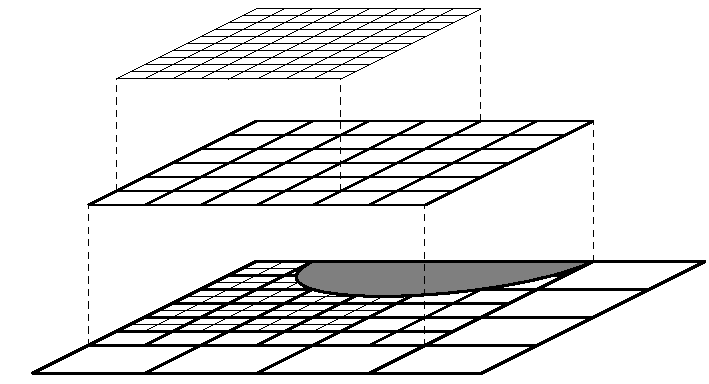
\includegraphics{./figures/amr2}
  \caption{Patch-based AMR. The figure shows two refined grids that hierarchically overlap a base grid. On each grid, boundary cells are cut by an external surface (shaded region).}
  \label{fig:patch_amr}
\end{figure}



We have implemented Eq.~\eqref{eq:minimal_plasma} into the Chombo library. In essence, Chombo is a library for performing patch-based AMR and also includes support for cut-cells. In addition, Chombo comes with some templated solvers (such as geometric multigrid), and several examples that can be used as stepping stones for more complex codes. 

\subsection{Spatial discretization}
Here, we give a brief summary to the spatial discretization. We discretize the physical domain by a set of Cartesian control volumes centered on points $\bmi = (i_0, \ldots, i_{\bm{D}-1})^\intercal \in \mathbb{Z}^{\bm{D}}$ where $\bm{D}$ is the dimension (typically, $\bm{D} = 2$ or $\bm{D} = 3$). Each control volume occupies the region $[\bmi - \frac{1}{2}\bm{u}\Delta x, \bmi + \frac{1}{2}\bm{u}\Delta x]$ where $\Delta x$ is a resolution and $\bm{u}$ is a vector whose components are all one (i.e. $\bm{u} = (1,1)^\intercal$ in 2D). Thus, a mesh $\Gamma\subset \mathbb{Z}^{\bm{D}}$ consists of a set of connected cells $\bmi \subset \Gamma$. Internal boundary conditions are resolved by cutting some of the cells with a level-set function $s(\bm{x}) = 0$ which describes the boundary interface. Inside each cut-cell, the boundary is linearized so that it intersects through the cell as a line in 2D, and a plane in 3D. Control volume faces that are cut by this surface are referred to as cut-faces, and the boundary itself is referred to as an embedded boundary (EB). More complex boundaries are built through constructive solid geometry (CSG) by using boolean operations such as unions, intersections, sums etc. Patch-based adaptive Mesh Refinement (AMR) is used by allowing recursively refined overlapping grids. We work with a set of grids $\Gamma^l$ that are nested hierarchically from the coarsest grid to the finest grid; the refinement factor between each level is always 2. We always require that a grid $\Gamma^l$ covers the overlapping region of a coarser grid $\Gamma^{l-1}$ and a finer grid $\Gamma^{l+1}$. Figure~\ref{fig:patch_amr} shows the grids in greater detail. 

Figure~\ref{fig:spatial_discretization} shows the the cut cells in greater details. Here, a cell is identified by it's index $\bmi$. We will take $\bm{x}_{\bmi}$ to be the \emph{cell center}, and $\overline{\bm{x}}_{\bmi}$ to the be \emph{cell centroid}. The volume fraction is $0 \leq \kappa_{\bmi} \leq 1$: Cells with $\kappa_{\bmi} = 0$ are denoted as \emph{covered} cells and lie completely outside the computational domain; cells with volume fractions $0 < \kappa_{\bmi} < 1$ are called \emph{irregular} cells and lie partially inside the computational domain (see e.g. the middle cell in Fig.~\ref{fig:spatial_discretization}). Furthermore, cell faces are denoted by $f^\pm_d(\bmi)$ where $\pm$ indicates the high ($+$) or low ($-$) face of the cell $\bmi$ in the coordinate direction $d$. A face center for face $f^\pm_d(\bmi)$ is therefore located at $\bm{x}_{\bmi \pm \frac{1}{2}\mathbf{e}_d}$ where $\mathbf{e}_d$ is a unit vector in the $d$-direction. Face centroids are likewise denoted $\overline{\bm{x}}_{\bmi \pm \frac{1}{2}\mathbf{e}_d}$ and the corresponding area fractions are denoted by $\alpha_{\bmi\pm\frac{1}{2}\bm{e}_d}$. Finally, the EB centroid is denoted by $\overline{\bm{x}}_{\bmi}^{\text{EB}}$ with a corresponding area fraction $\alpha^{\text{EB}}_{\bmi}$ and an outward normal vector $\bm{n}_{\bmi}$.

\begin{figure}[ht]
  \centering
  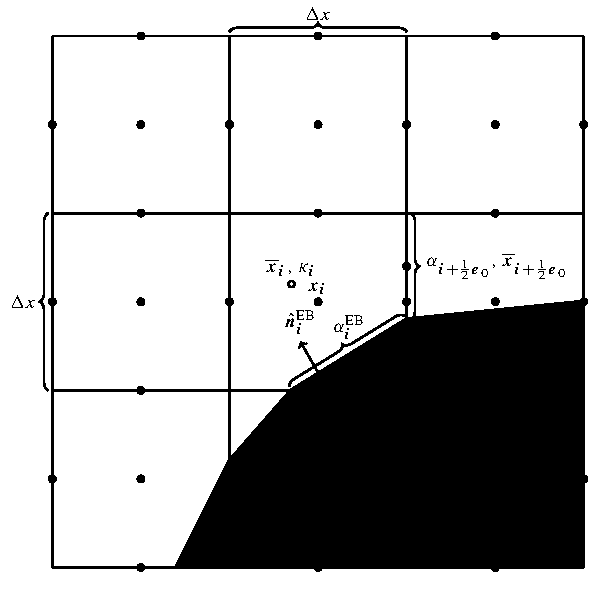
\includegraphics{./figures/spatial_discretization}
  \caption{Cut-cell discretization.}
  \label{fig:spatial_discretization}
\end{figure}

To derive the above quantities, let $V_{\bmi}$ denote the part of the Cartesian cell inside the computational domain, $A_{\bmi}^{\pm, d}$ be the un-cut part of a face $f^{\pm}_d(\bmi)$, and $A_{\bmi}^{\text{EB}}$ be the part of the EB that intersects with the cell. The above quantities are given by
\begin{subequations}
  \begin{align}
    \overline{\bm{x}}_{\bmi} &= \frac{1}{\Delta x^{\bm{D}}}\int_{V_{\bmi}}\bm{x}\diff V_{\bmi},\\
    \overline{\bm{x}}_{\bmi\pm\frac{1}{2}\bm{e}_d} &= \frac{1}{\Delta x^{\bm{D}-1}}\int_{A_{\bmi}^{\pm, d}}\bm{x}\diff A_{\bmi}^{\pm, d},\\
    \overline{\bm{x}}_{\bmi}^{\text{EB}} &= \frac{1}{\Delta x^{\bm{D}-1}}\int_{A_{\bmi}^{\text{EB}}}\bm{x}\diff A_{\bmi}^{\text{EB}}, \\
    \kappa_{\bmi} &= \frac{1}{\Delta x^{\bm{D}}}\int_{V_{\bmi}}\diff V_{\bmi},\\
    \alpha_{\bmi\pm\frac{1}{2}\bm{e}_d} &= \frac{1}{\Delta x^{\bm{D}-1}}\int_{A_{\bmi}^{\pm, d}}\bm{x}\diff A_{\bmi}^{\pm, d},\\
    \alpha_{\bmi}^{\text{EB}} &= \frac{1}{\Delta x^{\bm{D}-1}}\int_{A_{\bmi}^{\text{EB}}}\diff A_{\bmi}^{\text{EB}}, \\
    \bm{n}_{\bmi} &= \frac{1}{\Delta x^{\bm{D}-1}}\int_{A_{\bmi}^{\text{EB}}}\bm{n}\diff A_{\bmi}^{\text{EB}}.
  \end{align}
\end{subequations}

For brevity's sake, we will from now on omit the dependency on $\bmi$, and re-specify this when necessary.

\subsection{Poisson \& Eddington equations}
\label{sec:poisson}
We use the finite volume method for the Poisson equation and Eddington equations. For brevity, we restrict our discussion to the Poisson equation; the Eddington equations contain additional diagonal terms which can be added into the analysis below. Writing the Poisson equation in integral form yields
\begin{equation}
  \oint_A \epsilon\nabla\phi\cdot\diff\bm{A} = -\frac{1}{\epsilon_0}\int_V\rho\diff V
\end{equation}

\begin{figure}[ht]
  \centering
  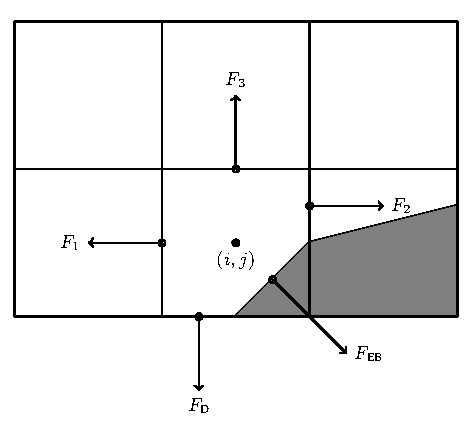
\includegraphics{./figures/cutCell}
  \caption{Cut cell at domain face.}
  \label{fig:cut_cell}
\end{figure}

As an example, we consider the cell shown in Fig.~\ref{fig:cut_cell}. Here, the volume $V_{\bmi}$ is a cut-cell at a domain boundary. Integration of Poisson's equation yields
\begin{equation}
  \oint_A \epsilon\nabla\phi\cdot\diff\bm{A} = F_1 + F_2 + F_3 + F_{\text{D}} + F_{\text{EB}},
\end{equation}
where the fluxes are centroid-centered on their respective faces. We use second order differences to discretize the face-centered fluxes. For example, for the flux through the top face in Fig.~\ref{fig:cut_cell} we find
\begin{equation}
  F_3 = F_{i,j+\nicefrac{1}{2}} = \epsilon_{i, j+\nicefrac{1}{2}}\frac{\phi_{i, j+1} - \phi_{i,j}}{\Delta x}.
\end{equation}
For fluxes through face centroids we interpolate face-centered to their centroids. For example, the flux $F_2$ in Fig.~\ref{fig:cut_cell} is given by
\begin{equation}
  F_2 = \alpha_{i+\nicefrac{1}{2}, j}\left[F_{i+\nicefrac{1}{2},j }(1-s) + sF_{i+\nicefrac{1}{2}, j+1}\right],
\end{equation}
where $s$ is the normalized distance from the face center to the face centroid, and $F_{i+\nicefrac{1}{2},j }$ and $F_{i+\nicefrac{1}{2}, j+1}$ are face-centered fluxes.

\subsubsection{Boundary conditions}
For Neumann boundary conditions the domain and embedded boundary fluxes are specified directly, whereas Dirichlet boundary conditions are more involved. For Dirichlet conditions on domain faces we apply finite differences in order to evaluate the flux. For example, for a constant Dirichlet boundary condition $\phi = \phi_0$, then the face-centered flux at the bottom face is, to first order,
\begin{equation}
  F_{i,j-\nicefrac{1}{2}} = -\epsilon_{i,j-\nicefrac{1}{2}}\frac{\phi_{i,j} - \phi_0}{\Delta x}. 
\end{equation}
Higher order boundary conditions are built by including more interior cells. Typically, we use second order boundary conditions in which
\begin{equation}
  F_{i,j-\nicefrac{1}{2}} = -\frac{\epsilon_{i,j-\nicefrac{1}{2}}}{\Delta x}\left(3\phi_{i,j+1} -\frac{1}{3}\phi_{i,j} - \frac{8}{3}\phi_0\right)
\end{equation}
As with the flux $F_2$ on the interior face, fluxes on domain faces are also interpolated to face centroids. Thus, $F_{\text{D}}$ becomes
\begin{equation}
  F_{\text{D}} = \alpha_{j-\nicefrac{1}{2}}\left[F_{i,j-\nicefrac{1}{2}}(1-t) + tF_{i-1,j-\nicefrac{1}{2}}\right],
\end{equation}
where $t$ is the distance from the face center to the face centroid.

\begin{figure}[ht]
  \centering
  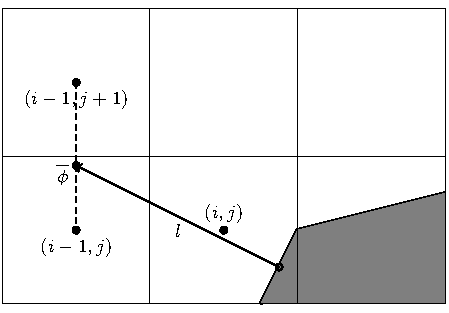
\includegraphics{./figures/raycast}
  \caption{Ray casting at the EB for obtaining the normal gradient. }
  \label{fig:raycast}
\end{figure}

The evaluation of Dirichlet boundary conditions on the EB is more complicated because the EB normal does not, in general, align with any of the coordinate directions. Various approaches for evaluating this term exist. Typically, we use a combination of two approaches. The first approach is a ray-casting method. Here, we cast a ray along the EB normal from the EB centroid into the domain and compute the intersection points between this ray and a line (plane in 3D) that connects two or more cell centers, see Fig.~\ref{fig:raycast}. At these points we interpolate the value of $\phi$ and then compute a finite difference approximation to the normal gradient. For example, to first order, the flux in \ref{fig:raycast} is
\begin{equation}
  F_{\text{EB}} = \alpha_{\text{EB}}\epsilon_{\text{EB}}\frac{\phi_{\text{EB}} - \overline{\phi}}{l},
\end{equation}
where $\overline{\phi}$ is the interpolated value at the intersection of the ray and the line that connects $\bm{x}_{i-1, j}$ and $\bm{x}_{i-1, j+1}$. 
Higher-order approximations to the flux can be built in a similar way by including more interior cells. Typically, we use second order boundary conditions. If we cannot find a stencil for computing the normal derivative this way, which can occur if there aren't enough cells available, we use least squares for computing the gradient. Before discussing least squares reconstruction, we mention that the Eddington equations require a boundary condition of the Robin type. Equation~\eqref{eq:robin} shows that the photon boundary flux is proportional to the solution at the boundary. Since this value is not known, we extrapolate it from the interior. On domain faces we simply use a first or second order finite difference approximation in order to extrapolate the solution from the interior to the domain face. Embedded boundaries require a more sophisticated approach which we discuss below. Typically, we use a second order Taylor-based finite difference stencil, which usually yields a comparatively compact stencil. If that fails we reconstruct the solution at the boundary by using weighted least squares, as discussed below. 

\paragraph{Least squares data reconstruction}

Our least squares methods are based on the minimization of a multidimensional Taylor series
\begin{equation}
  \phi_{\bm{i}} = \sum_{|q|\leq Q}\frac{1}{\bm{q}!}\left(\bm{x}_{\bm{i}} - \bm{x}_0\right)^{\bm{q}}\phi^{\bm{q}}(\bm{x}_0) + \mathcal{O}_{\bm{i}}\left(h^{Q+1}\right)
\end{equation}
where $h$ is the largest displacement $\left|\bm{x}_{\bm{i}} - \bm{x}_0\right|$ and $\bm{q}$ is a multi-index:
\begin{subequations}
  \begin{align}
    \bm{q}! &= q_1!q_2!q_3! \\
    \left(\bm{x}_{\bm{i}} - \bm{x}_0\right)^{\bm{q}} &= \left(x_1 - x_0\right)^{q_1}\left(x_2 - x_0\right)^{q_2}\left(x_3 - x_0\right)^{q_3}, \\
    \phi^{\bm{q}} &= \phi^{\bm{q}}(\bm{x}_0) = \frac{\partial^{q_1}}{\partial x_1^{q_1}}\frac{\partial^{q_2}}{\partial x_2^{q_2}}\frac{\partial^{q_3}}{\partial x_3^{q_3}}\phi\big|_{\bm{x}_0}.
  \end{align}
\end{subequations}

In the above, $\bm{x}_{\bm{i}}$ and $\phi_{\bm{i}}$ are known values, $\bm{x}_0$ is the point that we extrapolate to and $\phi^{\bm{q}}$ for $|\bm{q}| < Q$ are the unknown states at this point. We define a column vector of the unknown states $\Phi^{(Q)} = \left(\left\{\phi^{\bm{q}}\right\}\right)^\intercal$ and solve a system of equations by minimizing the residual
\begin{equation}
  \begin{split}
    f\left(\Phi^{\bm{Q}}\right) &= \sum_{\bm{i} \in \mathcal{N}}w_{\bm{i}}\mathcal{O}_{\bm{i}}^2\left(h^{Q+1}\right) \\
    &= \sum_{\bm{i} \in \mathcal{N}}w_{\bm{i}}\left[\phi_{\bm{i}} - \sum_{|q|\leq Q}\frac{1}{\bm{q}!}\left(\bm{x}_{\bm{i}} - \bm{x}_0\right)^{\bm{q}}\phi^{\bm{q}}(\bm{x}_0)\right]^2,
  \end{split}
\end{equation}
where $w_{\bm{i}}$ are weights and $\mathcal{N}$ is some neighborhood of cells (see Fig.~\ref{fig:lsq_neighborhood}). Typically, we weight with the inverse distance $w_{\bm{i}} = \left|\bm{x}_{\bm{i}} - \bm{x}_0\right|^{-1}$. We then minimize with respect to all unknown states, i.e. $\frac{\partial f}{\partial \phi^{\bm{p}}} = 0$, which yields $|\bm{p}| \leq Q$ equations in the form
\begin{equation}
  \sum_{\bm{i} \in \mathcal{N}}w_{\bm{i}}\frac{1}{\bm{p}!}\left(\bm{x}_{\bm{i}} - \bm{x}_0\right)^{\bm{p}}\left[\phi_{\bm{i}} - \sum_{|q|\leq Q}\frac{1}{\bm{q}!}\left(\bm{x}_{\bm{i}} - \bm{x}_0\right)^{\bm{q}}\phi^{\bm{q}}(\bm{x}_0)\right] = 0, \quad |\bm{p}| \leq Q.
\end{equation}

\begin{figure}[ht]
  \centering
  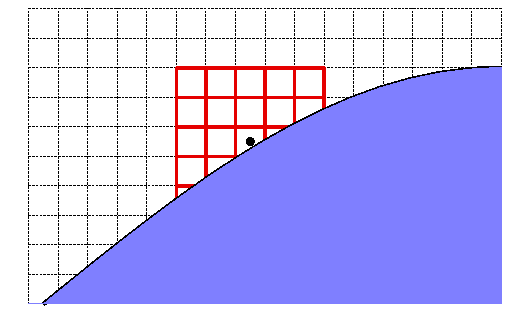
\includegraphics{./figures/lsq_neighborhood}
  \caption{Example neighborhood for least squares data reconstruction.}
  \label{fig:lsq_neighborhood}
\end{figure}

The above set of equations yields a linear system $\mathbb{A}\Phi^{(Q)} = \mathbb{B}\Phi^{(\mathcal{N})}$ where $\Phi^{(\mathcal{N})}$ is a column vector of the known values $\phi_{\bm{i}}$. In practice, we construct $\Phi^{(Q)}$, $\mathbb{A}$, and the rows of $\mathbb{B}$ in lexicographical order. For example, in two dimensions for Q = 2, we find
\begin{equation}
  \label{eq:q2_example}
  \Phi^{Q = 2} = 
  \begin{pmatrix}
    \phi_0 \\
    \partial_x\phi_0 \\
    \partial^2_x\phi_0 \\
    \partial_y\phi_0 \\
    \partial_{xy}\phi_0 \\
    \partial^2_y\phi_0
  \end{pmatrix}.
\end{equation}

The system of equations is solved by
\begin{equation}
  \Phi^{(Q)} = \left(\mathbb{A}^+\mathbb{B}\right)\Phi^{(\mathcal{N})},
\end{equation}
where $\mathbb{A}^+$ is the Moore-Penrose pseudoinverse. We compute this by first obtaining the singular value decomposition of $\mathbb{A} = \mathbb{V}\Sigma^+ \mathbb{U}^\ast$, which directly yields $\mathbb{A}^+ = \mathbb{U}\Sigma\mathbb{V}^\ast$.

Once $\mathbb{C} = \mathbb{A}^+\mathbb{B}$ is computed, we can obtain stencils for the entire unknown state $\Phi^{(Q)}$. The stencil for obtaining the interpolated value $\phi(\bm{x}_0)$ is found in the first row of $\mathbb{C}$. Likewise, for $Q=2$ in two dimensions, the stencil for the gradient is found in the second and fourth rows, respectively (see Eq.~\eqref{eq:q2_example}). 

\subsubsection{Multigrid solver}
The discretized Poisson equation is solved by embedding it in a geometric multigrid solver in residual-correction form. Multigrid involves iterative relaxation on progressively coarsened grids and is also compatible with AMR. On the coarsest level, the discretized system is solved directly with a biconjugate gradient stabilized method. Typically, better convergence for each cycle is achieved the further one coarsens; for domains without embedded boundaries one may coarsen up to a level where the domain only consists of two cells in one of the coordinate directions. However, for embedded boundary applications the multigrid convergence rate usually deteriorates when one coarsens too far. This occurs because, past a certain point, the coarse grid operator no longer well represents the longer wavelength modes of the fine grid operator (because the EB stencils have changed). Over-coarsening may also lead to geometrical under-resolution. We try to avoid these issues by dropping to the bottom solver prematurely; we usually drop to the bottom solver after 1-4 multigrid coarsenings of the coarsest grid. 

\subsection{Convection-Diffusion-Reaction equations}
For the mass transport equation we apply the method of Godunov with van Leer limiting to the equation:
\begin{equation}
  \frac{\partial n}{\partial t} = - \nabla\cdot(\bm{v}n) + \nabla\cdot\left(D\nabla n\right) + S.
\end{equation}
For the diffusive term $\nabla\cdot\left(D\nabla n\right)$ we use the discretization used for the Poisson and Eddigton equations. It is thus sufficient to discuss the construction of the advective term $\nabla\cdot(\bm{v}n)$. 

\subsubsection{Advective discretization}



\subsubsection{Hybrid divergence}
\label{sec:hybrid}
A problem with cut-cell grids is that the CFL condition on the time step is at best
\begin{equation}
  \Delta t = \mathcal{O}\left(\frac{\Delta x}{\bm{v}_{\bmi}^{\text{max}}}\kappa_{\bmi}^{\frac{1}{\bm{D}}}\right),
\end{equation}
which is the well-known small-cell problem with embedded boundary grids. The approach that we take to this problem is to stabilize the advective discretization by computing a hybrid discretization which expands the range of influence of small control volumes. Firstly, we compute the non-conservative divergence (i.e. which does not include the effect of the embedded boundary)
\begin{equation}
  \begin{split}
    \text{Div}^{\text{NC}}(F) &= \sum
  \end{split}
\end{equation}
Note that the computation of the non-conservative divergence requires second order solutions covered faces. The full algorithm for extrapolation can be found in [van Straalen, Graves: an adaptive cartesian grid embedded...]

Secondly, we compute the conservative divergence
\begin{equation}
  \begin{split}
    \text{Div}^{\text{NC}}(F) &= \sum 
  \end{split}
\end{equation}
We then use a hybridization of these two estimates in order to obtain a stable method:
\begin{equation}
  \nabla\cdot\left(\bm{u} n\right) = \kappa_{\bmi}\text{Div}^{\text{C}}(F) + \left(1 - \kappa_{\bmi}\right)\text{Div}^{\text{NC}}(F).
\end{equation}

The above method fails to conserve by the difference between the hybrid and conservative divergence,
\begin{equation}
  \delta M_{\bmi} = \kappa_{\bmi}\left(1-\kappa_{\bmi}\right)\left[\text{Div}^{\text{C}}(F) -\text{Div}^{\text{NC}}(F)\right]. 
\end{equation}
In order to maintain global conservation, this mass difference is redistributed into nearby cells,
\begin{equation}
  \nabla\cdot\left(\bm{u} n\right) \rightarrow \nabla\cdot\left(\bm{u} n\right) + w_{\bmi, \bmi^\prime}\delta M_{\bmi^\prime},
\end{equation}
where $w_{\bmi} > 0$ are weights which fulfill
\begin{equation}
  \sum_{\bmi^\prime \in N(\bmi)}w_{\bmi, \bmi^\prime}\kappa_{\bmi^\prime}
\end{equation}
where $N(\bmi)$ is a set of indices in the neighborhood of $\bmi$. We use volume weighted redistribution
\begin{equation}
  w_{\bmi, \bmi^\prime} = \frac{1}{\displaystyle\sum_{\bmi^\prime \in N(\bmi)}\kappa_{\bmi^\prime}}.
\end{equation}

\subsubsection{Refluxing and redistribution}
\label{sec:reflux}
If the embedded boundary does not cross a coarse-fine interface, straightforward refluxing at the coarse-fine interface is sufficient for closing the advective discretization. We do this by precomputing a set of flux registers that hold the face centered fluxes on both sides of the coarse-fine interface. Refluxing is then just a matter of subtracting the coarse flux from the divergence computation, and adding in the sum of the fine face fluxes. I.e. let $\{f_{\text{f}}(f_{\text{c}})\}$ be the set of fine faces that are obtained when coarsening of a coarse face $f_{\text{c}}$. In the reflux step, the divergence in the coarse cell is then modified as
\begin{equation}
  \nabla\cdot\bm{F} \rightarrow \nabla\cdot\bm{F} + \frac{1}{\Delta x}\left(\sum_{f} F_{f} - F_c\right),
\end{equation}
where $F_{c}$ and $F_{f}$ are the coarse and fine-face fluxes, and the sum runs over all the fine faces. 

If coarse-fine interfaces are allowed to cross the embedded boundary, the reflux-redistribution process is more complex since it must also account for mass moving between fine and coarse level. Thisf also involves ''re-redistribution'' where we correct the mass redistribution that was redistributed to the coarse grid from a fine grid.


\section{Temporal discretization}
We have implemented various explicit and semi-implicit discretizations for advancing the equations in time. We do not have an implicit solver, although work in that direction is ongoing. 

\subsection{Explicit 2nd order Runge-Kutta}
As a first step, we have chosen to integrate our equations of motion by using explicit, second order Runge-Kutta methods. For equations of the type
\begin{equation}
  \label{eq:ode}
  \frac{\partial f}{\partial t} = g,
\end{equation}
the second order Runge-Kutta method between time steps $k\Delta t$ and $(k+1)\Delta t$ is given by: 
\begin{equation}
  f^{k+1} = f^k + \Delta t\left[\left(1 - \frac{1}{2\alpha}\right)g^k + \frac{1}{2\alpha}g^{k+\alpha}\right].
\end{equation}
Here, $f^{k+\alpha}$ denotes the state at the intermediate time step $(k+\alpha)\Delta t$ where $\alpha$ denotes the Runge-Kutta method. For example, the midpoint and Heun's method (which is TVD) are given by $\alpha = 1/2$ and $\alpha = 1$, respectively. Note that the two-stage Runge-Kutta method requires two right-hand side evaluations for each time step, making it necessary to solve the Poisson and Eddington equations twice during a single time step.

Applying the above time stepping method to the minimal plasma model yields
\begin{subequations}
  \begin{align}
    n^{k+\alpha} &= n^k + \alpha\Delta t G^k, \\
    \sigma^{k+\alpha} &= \sigma^k + \alpha \Delta t F^k,
  \end{align}
\end{subequations}
where $G = S - \nabla\cdot(\bm{v} n) + \nabla\cdot(D\nabla n)$. These values then used to obtain new solutions for the Poisson and Eddington equations, which yields intermediate photon densities and fields $E^{k+\alpha}$, $\bm{E}^{k+\alpha}$ which are then used to advance the remaining fraction of the time step:
\begin{subequations}
  \begin{align}
    n^{k+1} &= n^k + \Delta t\left[\left(1 - \frac{1}{2\alpha}\right)G^k + \frac{1}{2\alpha}G^{k+\alpha}\right], \\
    \sigma^{k+1} &= \sigma^k + \Delta t\left[\left(1 - \frac{1}{2\alpha}\right)F^k + \frac{1}{2\alpha}G^{k+\alpha}\right].
  \end{align}
\end{subequations}
After the new densities and surface charges have been obtained, we re-evaluate the Poisson and Eddington equations at the end of the time step which yields the new values $E^{k+1}$, $\bm{E}^{k+1}$.

\subsection{4th order Runge-Kutta}
The classical fourth order Runge-Kutta method for \eqref{eq:ode} is
\begin{subequations}
  \begin{align}
    k_1 &= \Delta tG\left(t^k, n^k\right), \\
    k_2 &= \Delta tG\left(t^k+\frac{\Delta t}{2}, n^k + \frac{k_1}{2}\right), \\
    k_3 &= \Delta tG\left(t^k+\frac{\Delta t}{2}, n^k + \frac{k_2}{2}\right), \\
    k_4 &= \Delta tG\left(t^k+\Delta t, n^k + k_3\right), \\
    n^{k+1}  &= n^k + \frac{1}{6}\left(k_1 + 2k_2 + 2k_3 + k_4\right),
  \end{align}
\end{subequations}
and an equivalent equation is found for advancing $\sigma^k\rightarrow \sigma^{k+1}$. After evaluating each $k$, it is necessary to solve the Poisson and Eddington equations before evaluating the next one. For example, evaluation of $k_2$ requires the solution of the Poisson equation with the space charge density computed as $\rho = \sum q_n\left(n^k + \frac{k_1}{2}\right)$. 


\subsection{Semi-implicit TGA scheme}
We have also implemented a semi-implicit time stepping method. Our aim is to advance semi-implicitly by computing $\bm{v}$, $D$, and $S$ at half time steps, and then apply either a time-centered scheme (e.g. Crank-Nicholson). First, we decoupled the Poisson equation by solving it semi-implicitly at $t^{k+1/2}$. We do this by estimating variables explicitly at the half time step:
\begin{subequations}
  \begin{align}
    \widetilde{n}^{k+1/2} &= n^k + \Delta t G^k \\
    \widetilde{\sigma}^{k+1/2} &= \sigma^k + \Delta t F^k. 
  \end{align}
\end{subequations}
These values are then used to compute the Poisson and Eddington equations at the half time, i.e.
\begin{equation}
  \nabla\left(\epsilon\nabla\widetilde{\phi}^{k+1/2}\right) = -\frac{\rho^{k+1/2}}{\epsilon_0},
\end{equation}
where $\rho^{k+1/2} = \rho\left(\widetilde{n}^{k+1/2}, \widetilde{\sigma}^{k+1/2}\right)$. This essentially semi-implicitly decouples the elliptic equations from the hyperbolic ones, yielding
\begin{subequations}
  \begin{align}
    \partial_t n &= -\nabla\cdot\left(\widetilde{\bm{v}}^{k+1/2}n\right) + \nabla\cdot\left(\widetilde{D}^{k+1/2}n\right) + \widetilde{S}^{k+1/2}, \\
    \partial_t \sigma &= F\left(\widetilde{\bm{E}}^{k+1/2}, \widetilde{n}^{k+1/2}, \widetilde{E}_\nu^{k+1/2}\right).
  \end{align}
\end{subequations}




%% \subsection{2nd order implicit methods}
%% Direct numerical simulations of the minimal plasma model have shown that explit intregration of the equations of motion are sensitive to the timestep even if it is smaller the Courant-Friedrichs-Lewy condition. The reason for this is the feedback mechanism that is supplied through the plasma model which tends to reinforce numerical extrema. Often, and, especially for streamers that move along dielectric surfaces, the dielectric relaxation time is the limiting factor. We have also implemented an implicit multistep method which is iterated to convergence by using a predictor-corrector routine with functional iteration. 

%% First, we predict a value at the end of the time step by using explicit Euler integration
%% \begin{subequations}
%%   \begin{align}
%%     n^p      &= n^k + \Delta t G^k, \\
%%     \sigma^p &= \sigma^k + \Delta t F^k, \\
%%     \phi^p   &= \phi^p(n^p, \sigma^p), \\
%%     E^p      &= E^p(n^p, \sigma^p),
%%   \end{align}
%% \end{subequations}
%% where we drop species subscripts for brevity. Then, we correct these values by using the second order Adams-Moulton method (i.e. the implicit trapezoidal method):
%% \begin{subequations}
%%   \begin{align}
%%     n^c      &= n^k + \frac{\Delta t}{2}\left(G^p + G^k\right), \\
%%     \sigma^c &= \sigma^k + \frac{\Delta t}{2}\left(F^p + F^k\right), \\
%%     \phi^c   &= \phi^c(n^c, \sigma^c), \\
%%     E^c      &= E^c(n^c, \sigma^c). 
%%   \end{align}
%% \end{subequations}

%% We accept the corrected values if the system has converged properly, i.e. 
%% \begin{subequations}
%%   \begin{align}
%%     \left|n^c - n^p\right|           &< \lambda\left|n^p\right|, \\
%%     \left|\sigma^c - \sigma^p\right| &< \lambda\left|\sigma^p\right|.
%%   \end{align}
%% \end{subequations}
%% If the corrected values do not fulfill the above constraints, we set the predicted values to be equal to the corrected values and re-iterate. We exit only the predictor-corrector loop and set $n^{k+1} = n^c$ if the system has converged, or we exceed a maximum number of iterations. The whole system is therefore required to converge simultaneously. 
  

\subsection{Time step restrictions}
Multiple time step constraints are put in place in our code in order to ensure numerical stability, and accurate temporal evolution of the plasma as a whole. Firstly, the time step is restricted according to the CFL condition
\begin{equation}
  \Delta t_{\text{CFL}} = \alpha_{\text{CFL}}\text{Min}\left(\text{Min}_d\left(\frac{\Delta x}{u_d}\right), \frac{\Delta x^2}{2\bm{D}_{\text{max}}}\right),
\end{equation}
where $\alpha_{\text{CFL}}$ is the CFL number which we use for fine-tuning the time step. For explicit integration $\alpha_{\text{CFL}} < 1$, but this is not a contraint for our implicit integrator. 

In addition to the above two requirements, the electric field should evolve slowly across a single time step. We estimate a largest possible time step by applying explicit Euler integration to Ampere's law: 
\begin{equation}
  \epsilon_0\frac{\partial \bm{E}}{\partial t} = -\bm{J},
\end{equation}
We then discretize $\partial_tE_d = (E_d^{k+1}-E_d^k)/\Delta t$ which yields the dielectric relaxation time
\begin{equation}
  \Delta t_\epsilon = \alpha_{\epsilon}\text{Min}_d\left(\frac{\epsilon_0E_d}{J_d}\right),
\end{equation}
where the $\text{Min}_d$ operator runs over all spatial directions $d$. Again, $\alpha_{\epsilon}$ is a fudge-factor used for controlling the time step.

Finally, we restrict the time step by 
\begin{equation}
  \Delta t = \text{Min}\left(\Delta t_{\text{CFL}}, \Delta t_\epsilon\right).
\end{equation}

Note that we never ''backtrack'' in a simulation; if the time step yields a fractional increase which is larger than e.g. $\alpha_\epsilon$ (which can happen due to the use of multistep methods), we simply accept the result rather than backtracking to the previous time step.


\section{Numerical examples}
\label{sec:examples}
In this section we provide a few numerical examples that demonstrate the use of cut-cell grids for plasma simulations. For simplicity, we use well-established plasma kinetic models and restrict our discussions to comparatively simple geometries. %In section~\ref{sec:triple2D} we simulate a planar discharge that evolves from a wall protrusion near a dielectric surface. Section~\ref{sec:noise2D} simulates inception and propagation of a streamer from a needle-like electrode with the inclusion of surface roughness.

\subsection{Simplified bulk plasma kinetics}
We use the Morrow-Lowke plasma model for air and flue gases. The conservation equations that we solve are
\begin{subequations}
  \begin{align}
    \frac{\partial n_e}{\partial t} + \nabla\cdot(\bmu_en_e) - \nabla\cdot(D_e\nabla n_e) &= S_e, \\
    \frac{\partial n_+}{\partial t} + \nabla\cdot(\bmu_+n_+) -  &= S_+, \\
    \frac{\partial n_-}{\partial t} + \nabla\cdot(\bmu_+n_-) -  &= S_-, \\
  \end{align}
\end{subequations}
where $n_e$ is the electron density and $n_\pm$ are the positive and negative ion densities. The source terms are
\begin{subequations}
  \begin{align}
    S_e &= \alpha n_e\left|\bmu_e\right| - \eta n_e\left|\bmu_e\right| - \beta_{\text{e,+}}n_en_+ + S_{\text{ph}},\\
    S_+ &= \alpha n_e\left|\bmu_e\right| - \beta_{\text{e,+}}n_en_+ - \beta_{\text{+,-}}n_+n_- + S_{\text{ph}}, \\
    S_- &= \eta n_e\left|\bmu_e\right| - \beta_{\text{+,-}}n_+n_-,
  \end{align}
\end{subequations}
where $\alpha$ is the Townsend ionization coefficient, $\eta$ the Townsend attachment coefficient, $\beta_{\mu,\mu^\prime}$ the recombination coeffcient of two species $\mu$, $\mu^\prime$. Finally, $S_{\text{ph}}$ is the photoionization source term discussed below. Several of the quantities above are field-dependent; for example, the electron velocity is given by $\bmu_e = -\mu_e\bm{E}$ where $\mu_e$ is the electron mobility. The ionization and attachment coefficients $\alpha$ and $\eta$ are also field dependent, and so is the electron diffusion coefficient. Expressions for these may be found in Morrow-Lowke[citation neeeded]. 

In addition to the above reactions, we consider a three-group Eddigton SP1 photoionization model. That is, for $\gamma = 1, 2, 3$ we solve
\begin{equation}
  \nabla\cdot\left(\frac{1}{3\kappa_\gamma}\nabla E_\gamma\right) - \kappa_\gamma E_\gamma = \frac{\eta_\gamma}{c}. 
\end{equation}
The corresponding absorption lengths are $\kappa_\gamma = \lambda_\gamma p_{O_2}$ where $\lambda_1 = 4.15\times 10^{-2}\,\text{mPa}^{-1}$, $\lambda_2 = 1.09\times 10^{-1}\,\text{mPa}^{-1}$, and $\lambda_3 = 6.69\times 10^{-1}\,\text{mPa}^{-1}$. We use the same source term for each equation:
\begin{equation}
  \eta_\gamma = \frac{p_q}{p + p_q}\frac{\nu_e}{\nu_i}\alpha n_e\left|\bm{v}_e\right|,
\end{equation}
where the factor $p_q/(p+p_q)$ accounts for collisional quenching of an excited species of molecular nitrogen, and $\nu_e/\nu_i$ is the ratio between the electron impact excitation rate of $N_2$ and the electron impact ionization rate of $N_2$. Following Bourdon et. al we take $\nu_e/\nu_i = 0.6$.

The photoionization source term is given by a weighted sum of the solution for $E_\gamma$:
\begin{equation}
  S_{\text{ph}} = \sum_{\gamma = 1}^3 \xi_\gamma c p_{\text{O}_2}A_\gamma E_\gamma,
\end{equation}
where $\xi_\gamma$ is the photoionization efficiency, taken to be $\xi_\gamma = 0.1$ for simplicity. The coefficients $A_\gamma$ are weighting coefficients that are adapted to fit with the original Zheleznyak integral model, and are given by $A_1 = 1.12\times 10^{-4}\,\text{mPa}^{-2}$, $A_2 = 2.88\times 10^{-3}\,\text{(mPa)}^{-2}$, and $A_3 = 2.76\times 10^{-1}\,\text{(m\,Pa)}^{-2}$.

\subsubsection{Dielectric boundary conditions}
Electron emission from dielectric surfaces can occur through a number of different field-dependent process such as ion-bombardment, secondary electron impact, photoemission and field field-induced emission, to name a few. We consider a simple model for surface emission which consists of photoemission and ion bombardment. Photoemission is implemented by taken the influx of electrons from surface to be proportional to the outflux of photons into the dielectric. The Robin boundary condition for the Eddington equations has already been discussed [recall Eq.~\eqref{eq:photon_outflux}], so the influx of electrons is
\begin{equation}
  F_e = F_{e, \text{pe}} + F_{e, +},
\end{equation}
where $F_{e, \text{pe}}$ and $F_{e, +}$ are fluxes due to photoemission and positive ion bombardment, respectively. 

The photoemission term is given by
\begin{equation}
  F_e, {\text{pe}} = \begin{cases}
    -\gamma_{\text{pe}}\frac{c}{2}\sum_{\gamma = 1}^3 E_\gamma, & \bm{E}\cdot\bm{n} < 0,\\
    0, & \bm{E}\cdot\bm{n} \geq 0,
  \end{cases}
\end{equation}
where $\gamma_{\text{pe}}$ is the photoemission coefficient. The conditional clause is included because photo-emission is only possible in an external field that drives electrons away from the surface. 

In the same way, we model inflow of electrons by electron bombardment by
\begin{equation}
  F_{e, +} = \begin{cases}
    -\gamma_+F_+ & \bm{E}\cdot\bm{n} < 0,\\
    0, & \bm{E}\cdot\bm{n} \geq 0,
  \end{cases}
\end{equation}
where $F_+$ is the positive ion outflux on the dielectric and $\gamma_+$ is the second Townsend coefficient.

\subsection{Razor-blade gaps}
First, we consider examples of 

\subsection{Triple-junction setups}
\label{sec:triple2d}
Here, we consider the inception of a streamer on a wall protrusion and its connection to a dielectric surface. The geometry, initial mesh and field distribution is shown in Fig.~\ref{fig:triplePoint2D}.
\begin{figure}[ht]
  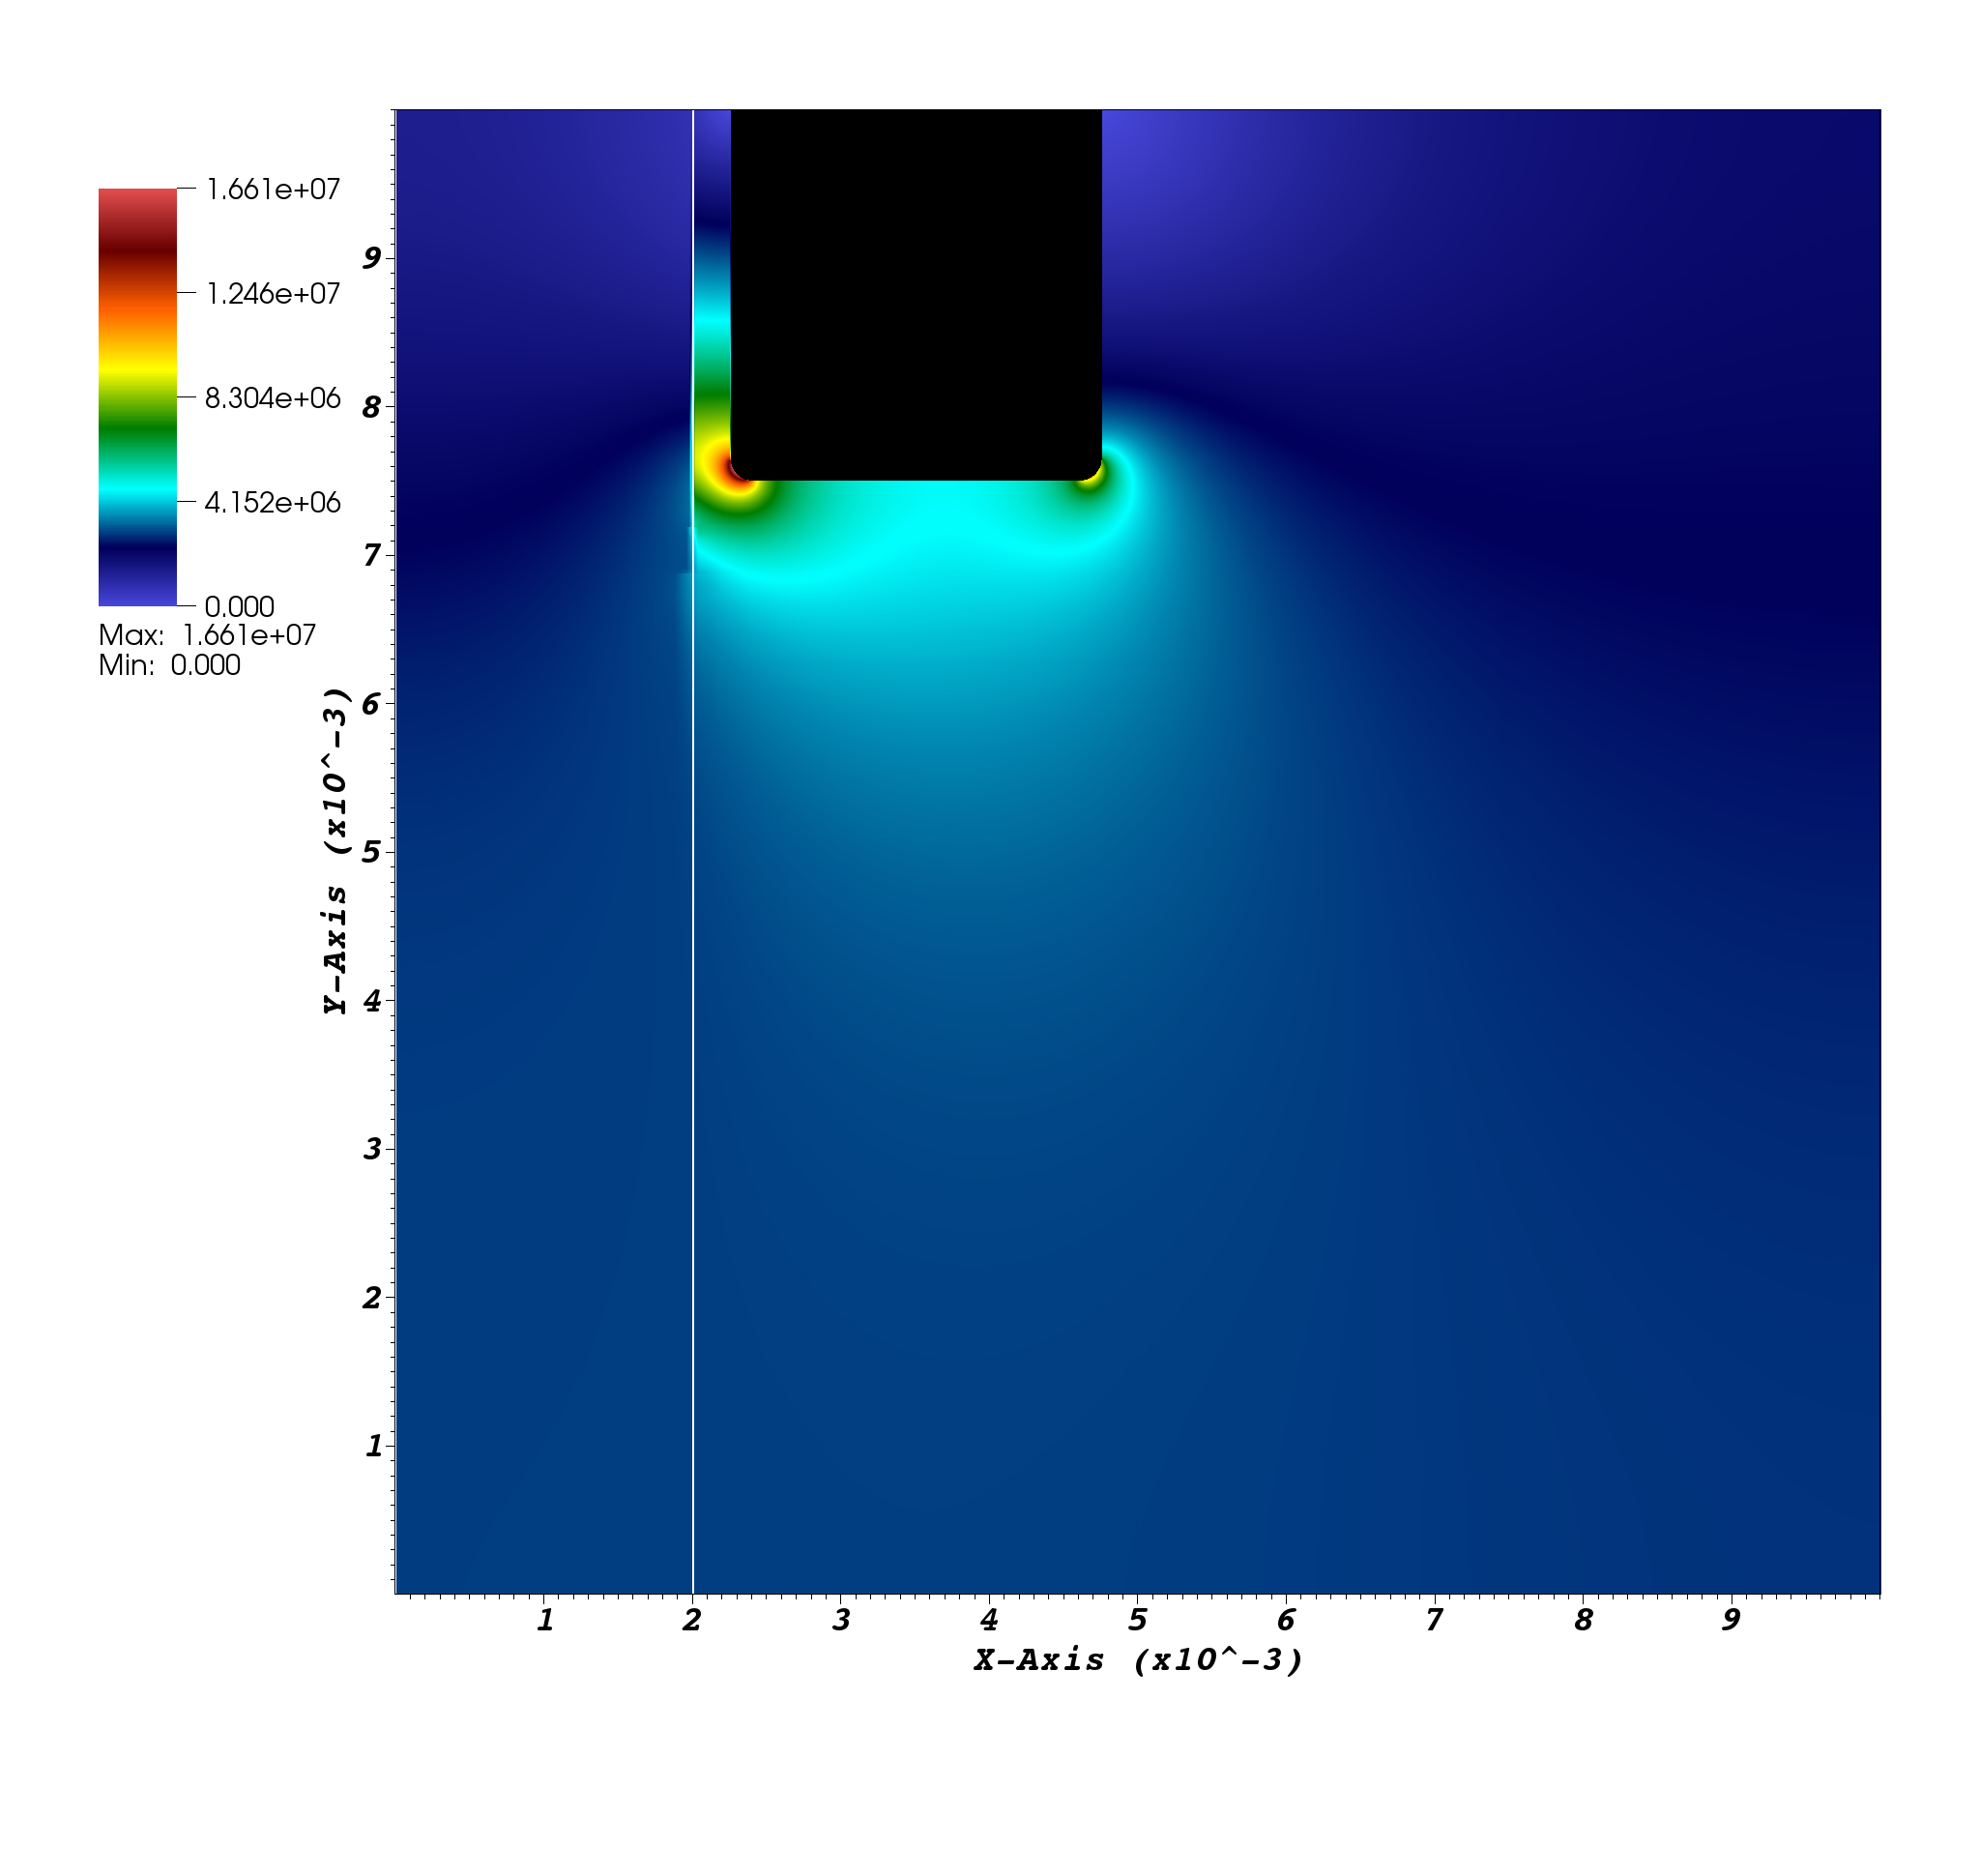
\includegraphics[width=.45\textwidth]{./figures/triplePoint2d/t0_big}
  \hfill
  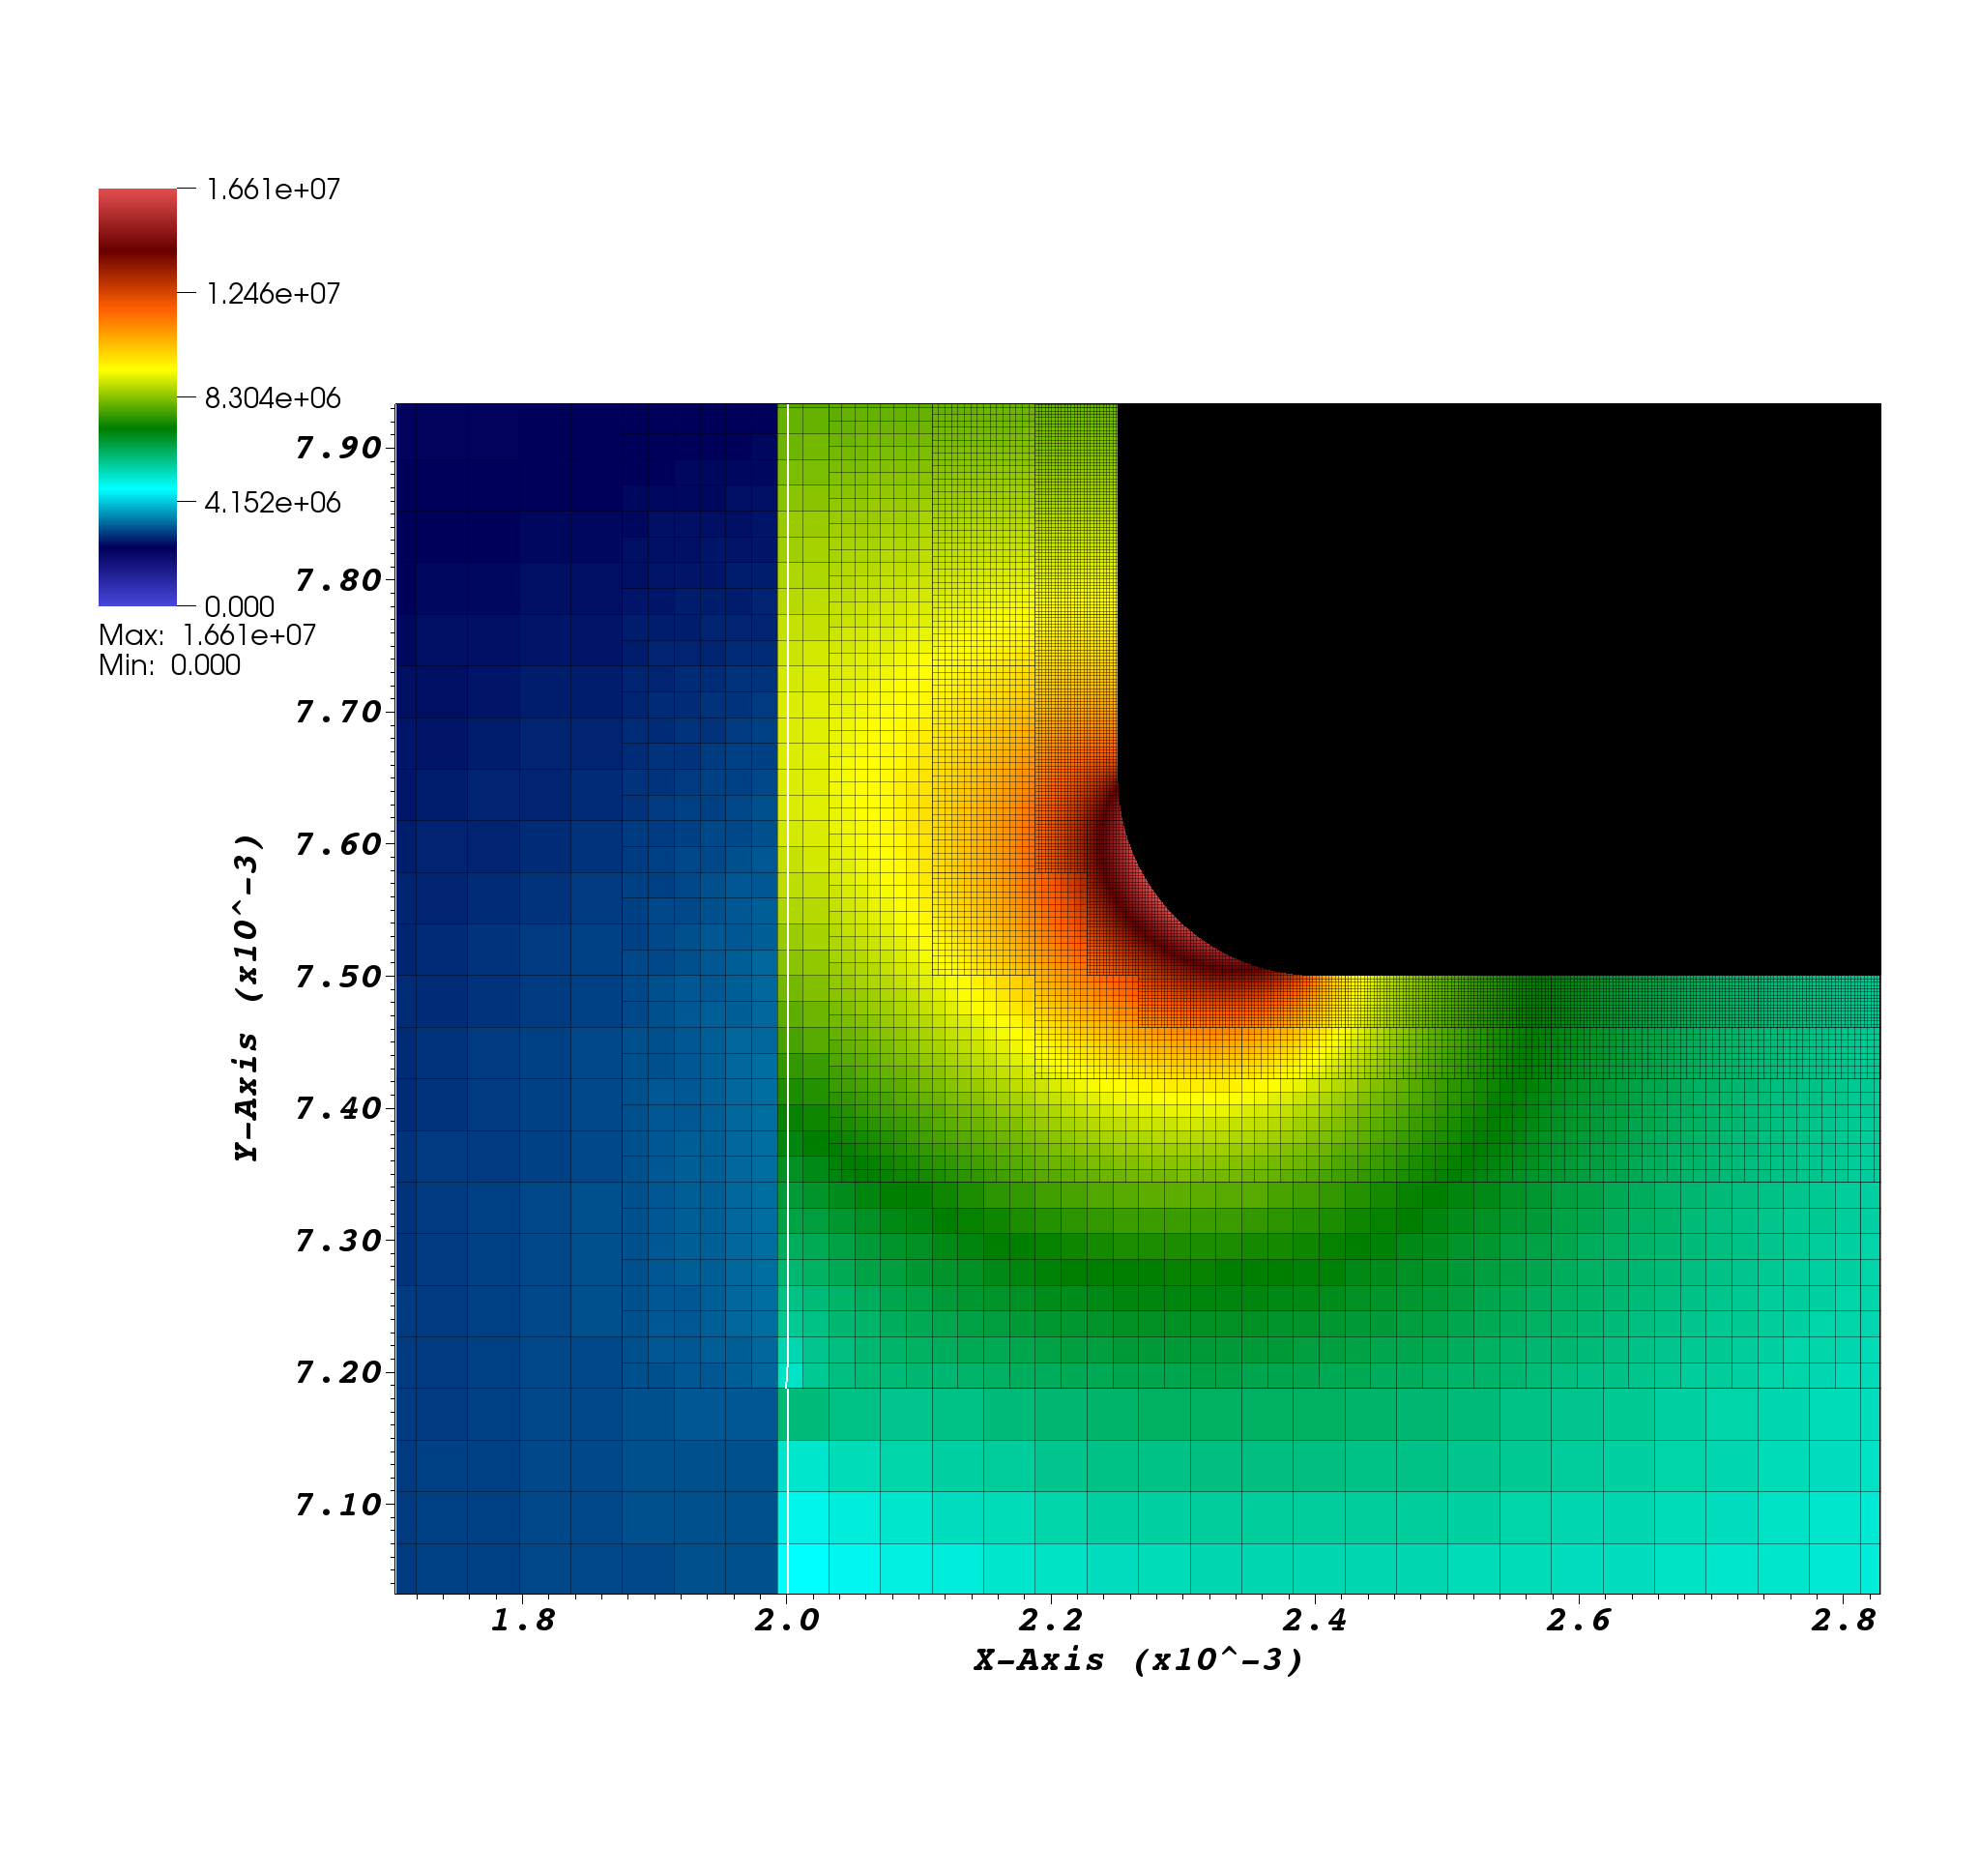
\includegraphics[width=.45\textwidth]{./figures/triplePoint2d/t0_small}
  \caption{Geometry and initial field distribution for a ''triple-junction'' setup.}
  \label{fig:triplePoint2d}
\end{figure}

\subsection{Streamer propagation from non-smooth electrodes}
\label{sec:noise2d}
In this section we consider inception and propagation of a positive streamer from an needle-like electrode. The electrode is a cylinder with a rounded cap at the end. The length and radius of the cylinder are $L = $ and $R = $.

We incorporate surface roughness of the electrode by displacing the level-set electrode surface with a noise function. We use Ken Perlin's algorithm for creating landscape noise. The backbone of this algorithm is the creation of random gradients at various cell nodes across a mesh. This is mesh is not related to the AMR grids on which our equations are solved. For a given position $\bm{x}$ we find the control volume which contains this cell and then compute the dot product between the displacement vector to each cell node and the gradient at the those nodes. Interpolation of these four nodal values (8 in 3D) then yield a pseudorandom smooth noise inside the cell. Several improvements to this algorithm exist. For example, we use the improved Perlin noise model which uses a randomly permuted hash table for selecting gradient directions, and an improved interpolant that removes some artifacts on the noise landscape. Figure~\ref{fig:perlin} shows typical examples of Perlin noise. 

\begin{figure}[ht]
  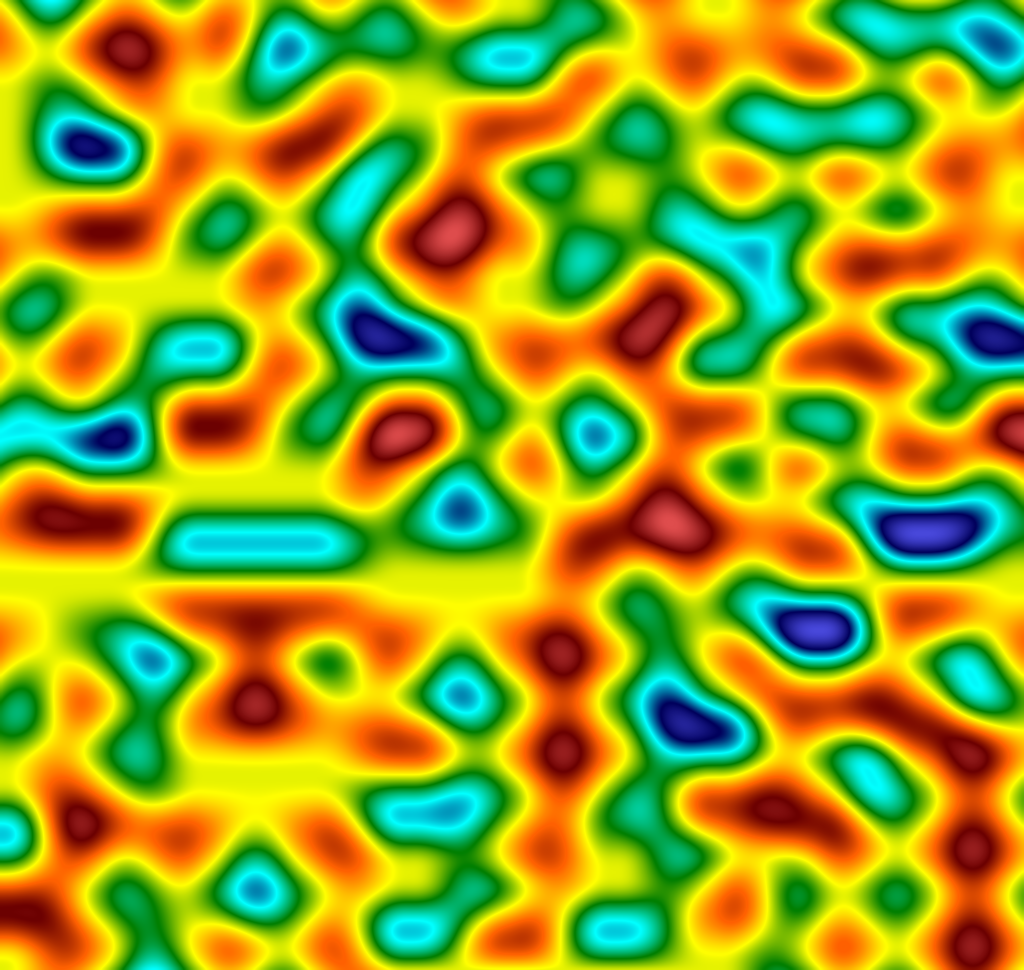
\includegraphics[width=.3\textwidth]{./figures/perlin1}
  \hfill
  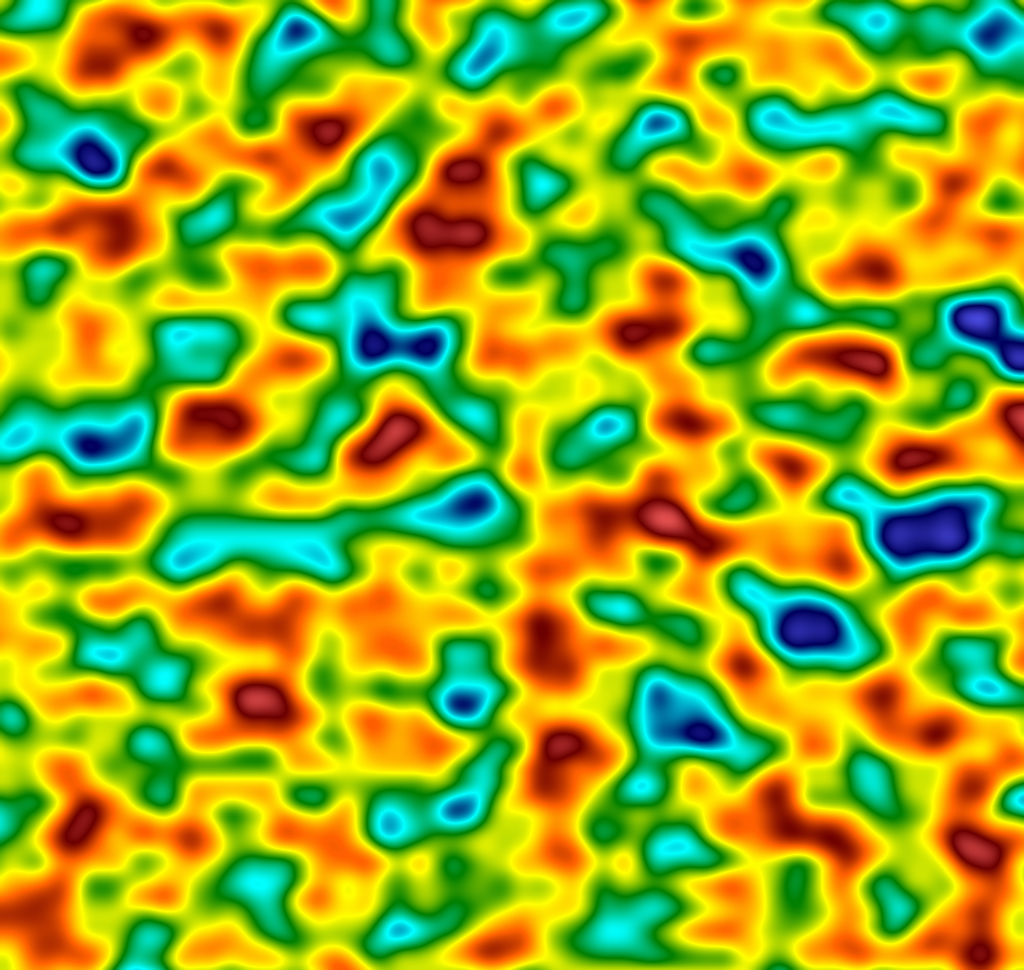
\includegraphics[width=.3\textwidth]{./figures/perlin2}
  \hfill
  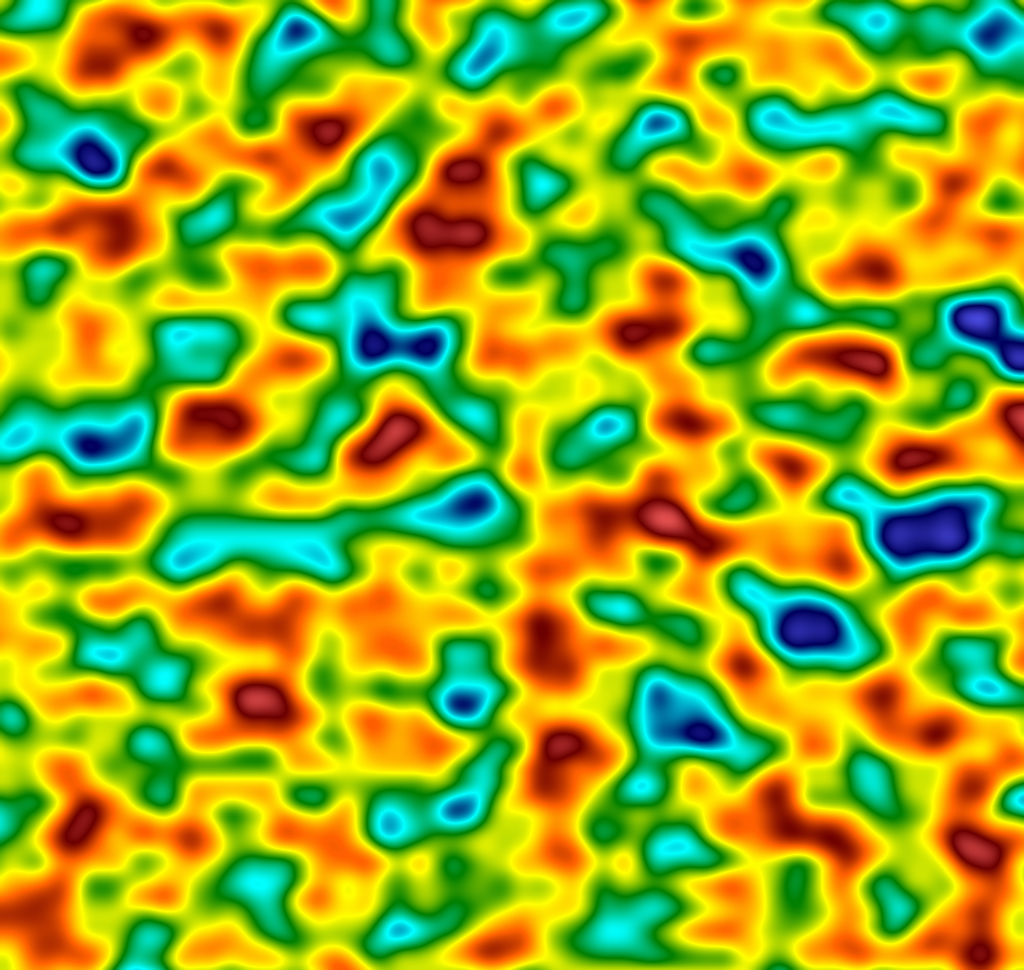
\includegraphics[width=.3\textwidth]{./figures/perlin2}
  \caption{Perlin noise across a domain (-1, 1). The base frequency is $\bm{k} = 5\left(\hat{\bm{x}} + \hat{\bm{y}}\right)$. Left: One octave. Middle: Two octaves. Right: Three octaves. }
  \label{fig:perlin}
\end{figure}

We use three octaves of Perlin noise folded in on itself. The spatial base frequency is $\bm{k} = 10^3\left(\hat{\bm{x}} + \hat{\bm{y}}\right)$ and the base amplitude is $20\,\mu\text{m}$. For each octave that we add the spatial frequency is doubled and the amplitude is reduced by a factor of 2. For reproducibility, the gradient permutation vector is kept equal to Ken Perlin's original one (i.e. we do not reseed the noise functions). This function is then used to intersect the level-set function of a cylinder with a hemisphere at its tip.

\begin{figure}[ht]
  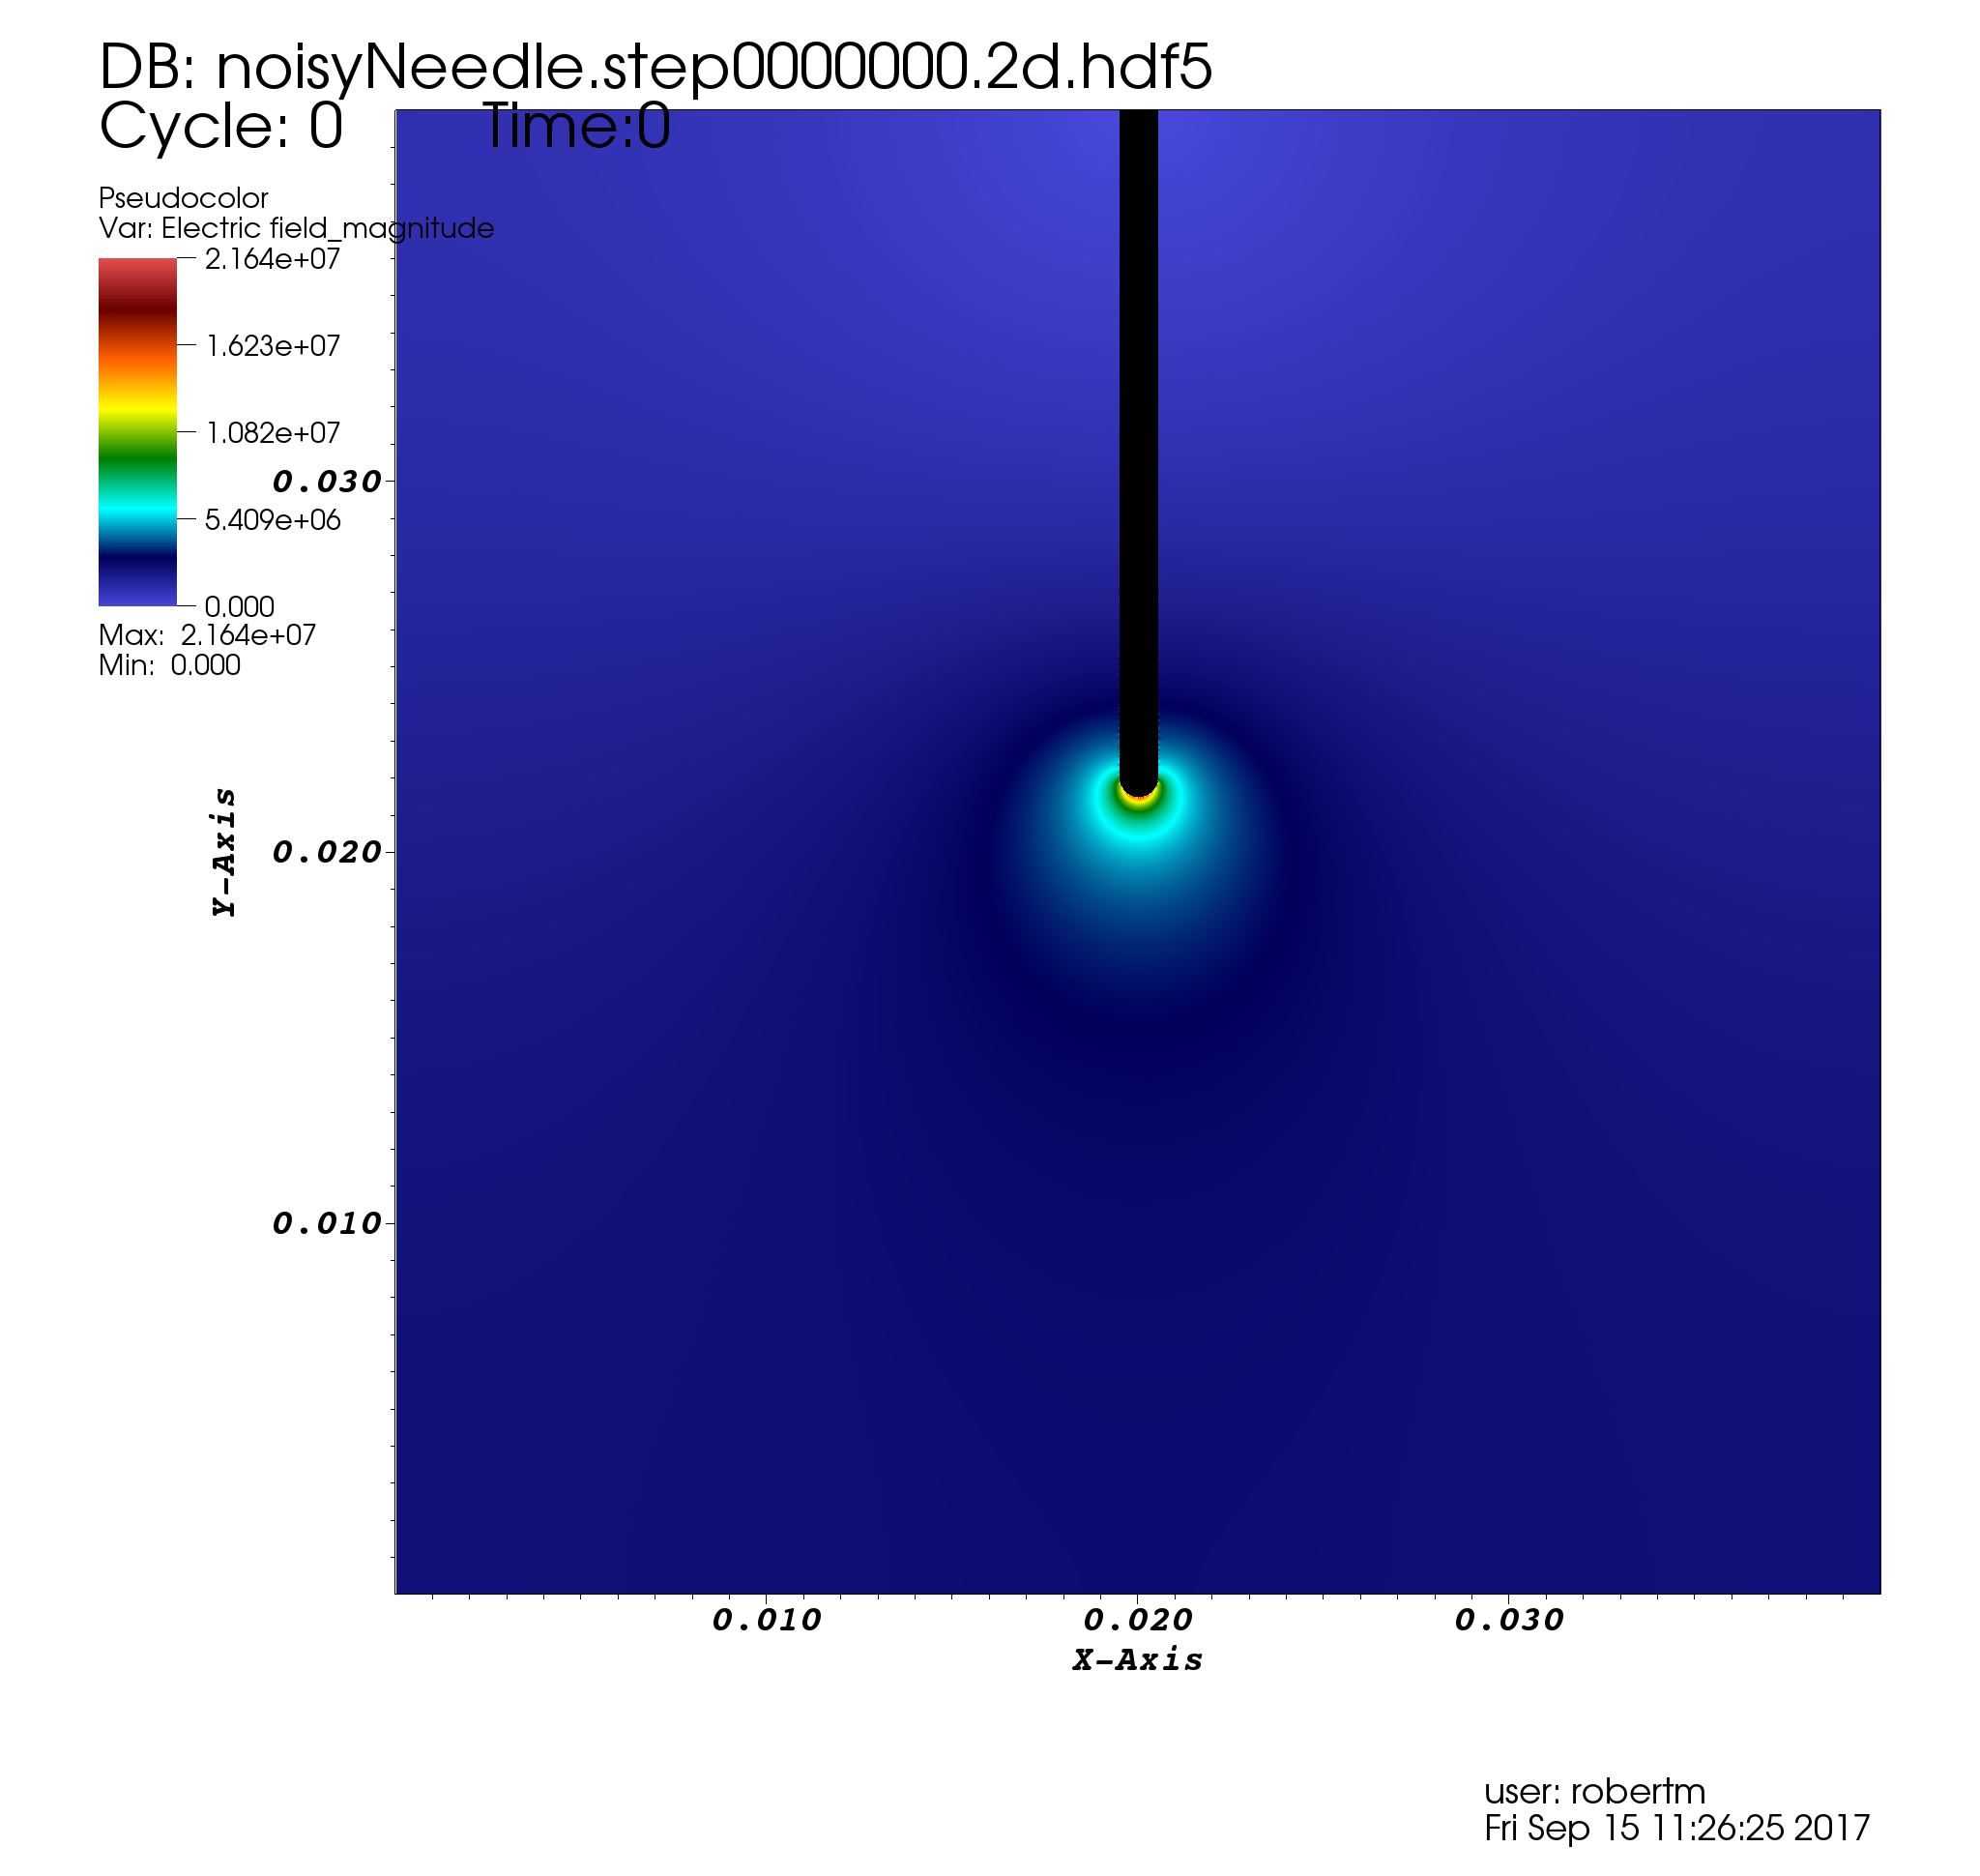
\includegraphics[width=.45\textwidth]{./figures/noisyCylinder/needle_big_t0}
  \hfill
  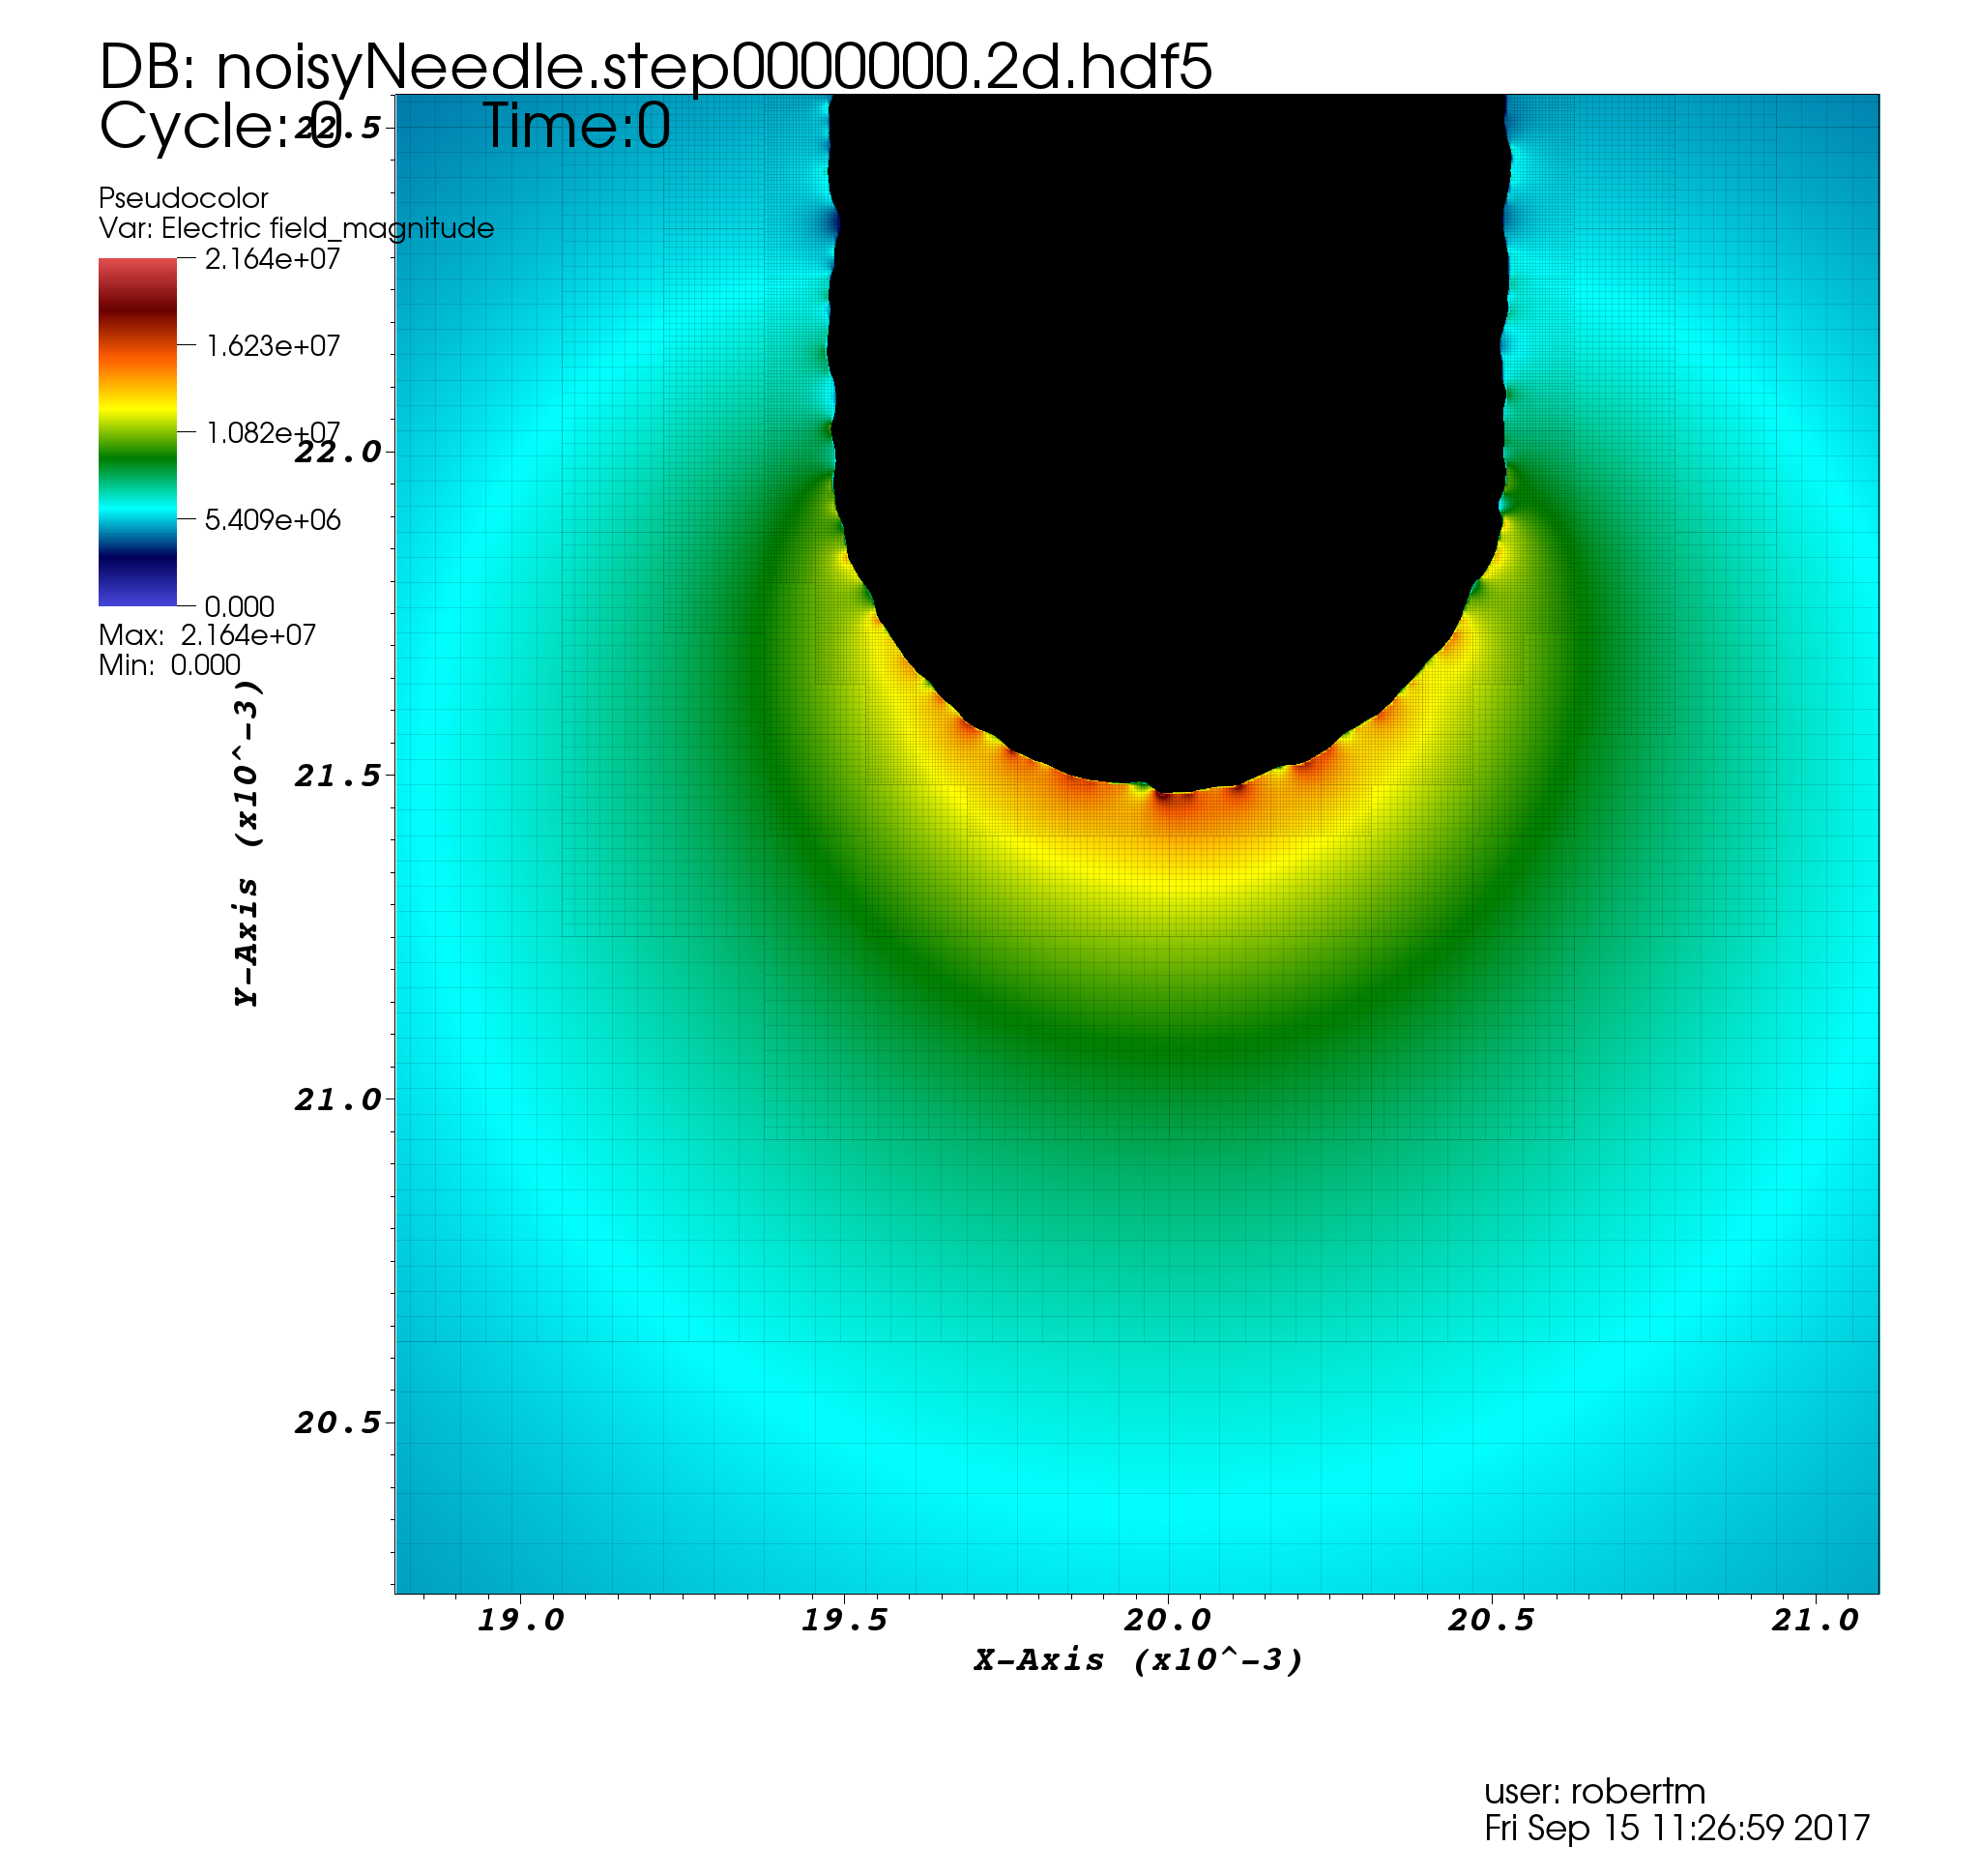
\includegraphics[width=.45\textwidth]{./figures/noisyCylinder/needle_small_t0}
  \caption{Cylindrical rod with surface roughness. Left: Electric field magnitude over the full domain. }
  \label{fig:roughCylinder}
\end{figure}

The computation domain is a $4\,\text{cm} \times 4\,\text{cm}$ and the needle protrudes $2\,\text{cm}$ from the top edge of the domain (see Fig. ~\ref{fig:roughCylinder}. For Poisson's equation we use a constant-voltage Dirichlet boundary conditions on the needle and the top edge. A homogeneous Dirichlet boundary condition is applied on the bottom plate, and homogeneous Neumann boundary conditions are applied on the left and right domain edges.

For the charged species we apply, for simplicity, an outflow condition on the domain edges. On the needle surface we apply outflow boundary conditions for electrons and negative ions if $\bm{E}\cdot\bm{n} > 0$ (i.e. the needle is an anode) and a wall boundary condition (i.e. zero-flux) for positive ions. For the 


\section{Concluding remarks}
\label{sec:remarks}


%\section{Conclusions}

\section*{Acknowledgements}
This work was financially supported by the Norwegian Research Council, ABB Skien, and ABB CRC. The author expresses his gratitude to D. T. Graves for advice on the Chombo infrastructure, and S. Pancheshnyi for fruitful discussions regarding plasma kinetics. 

\end{document}
